\chapter{Розповсюдження випромінювання плаского диску в нелінійному середовищі}
\label{ch:nonlinear}

%%%%%%%%%%%%%%%%%%%%%%%%%%%%%%%%%%%%%%%%%%%%%%%%%%%%%%%%%%%%%%%%%%%%%%%%%%%%%%%%
\section{Вторинне джерело поля в слабкому нелінійному середовищі. 
Нелінійність Керра}

При взаємодії з середовищем поле змінюється. Така повединка називається ефектом 
самодії. Джерелом такого поля стає весь простір його розповсюдження. Назвемо 
таке джерело вторинним. Випадки коли вторинним джерелом можна знехтувати, за 
рахунок його незначного вливу порівняно з первинним джерелом, називається 
лінійною задачею випромінювання. Прикладами такого поля є 
\eqref{eq:linear_h_cyl} та \eqref{eq:linear_e_cyl}. Тепер розглянемо 
середовище, де вплив самодії все ще незначний порівнянно з лінійним полем, але
викликає розбіжності в емпіричних показниках та данних теоретичної моделі. 
Таке середовище називають слабним нелінійним середовищем. Вторинне джерело 
поля в такому середовищі є функцією амплатуди поля. В якості такого джерела 
розглянемо вторинній електричний струм
%
\begin{equation*} 
\vect{J^\prime} = \partder{}{t} \vect{P^\prime} \left( \vect{E} \right)
\end{equation*}
%
\begin{figure}
    \centering
    \subfloat[A0=1 A/m]{{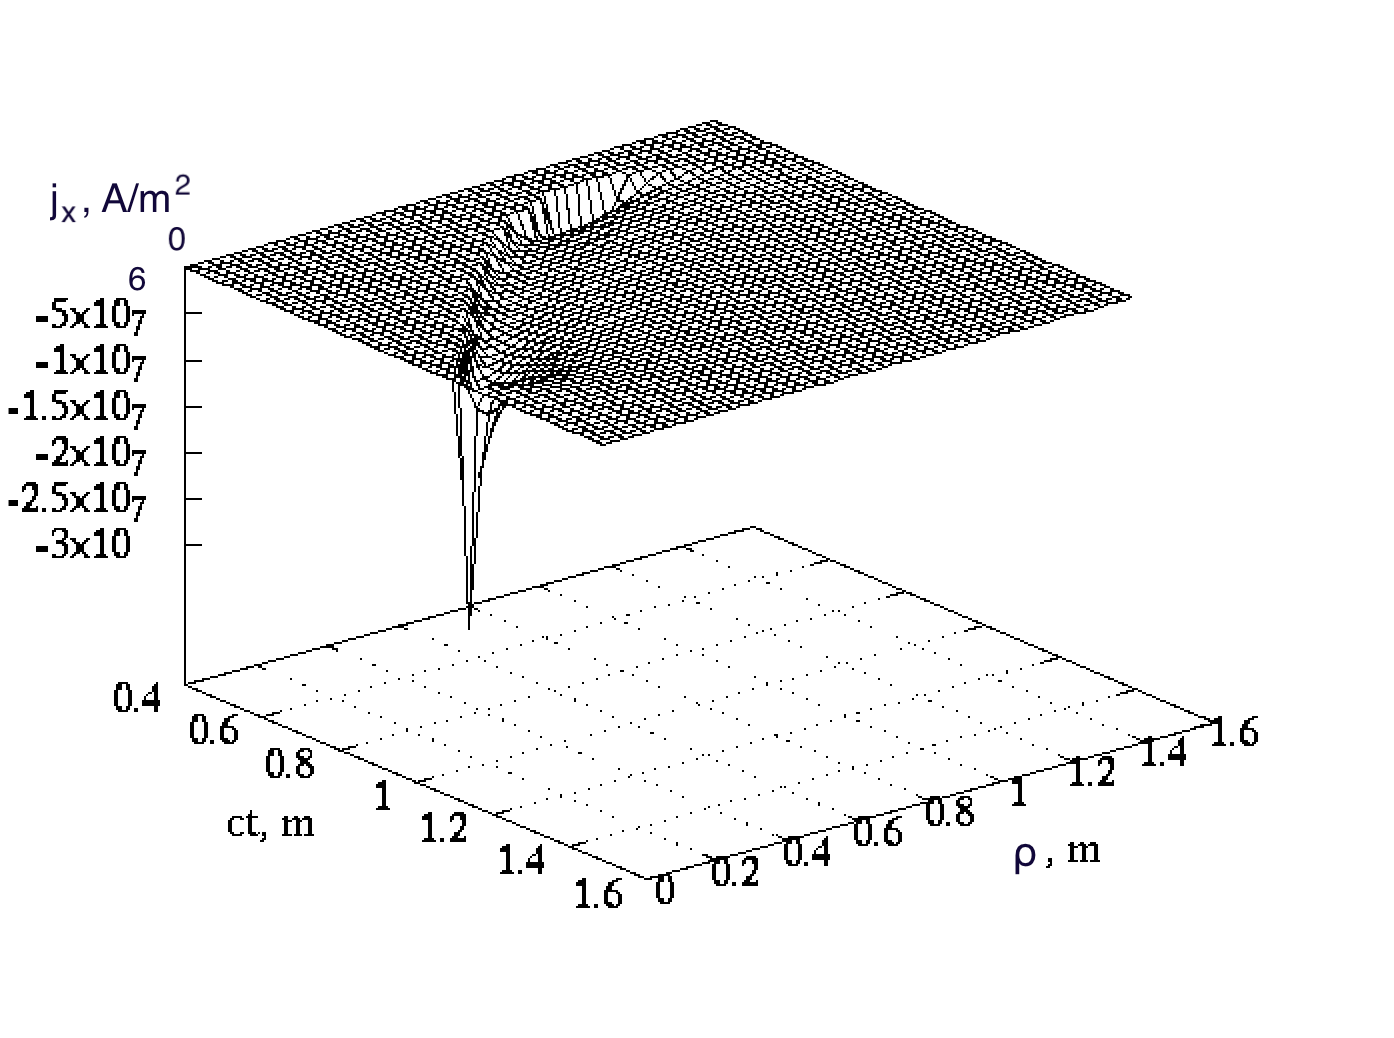
\includegraphics[width=5cm]{Jperp_A1} }}%
    \qquad
    \subfloat[A0=2 A/m]{{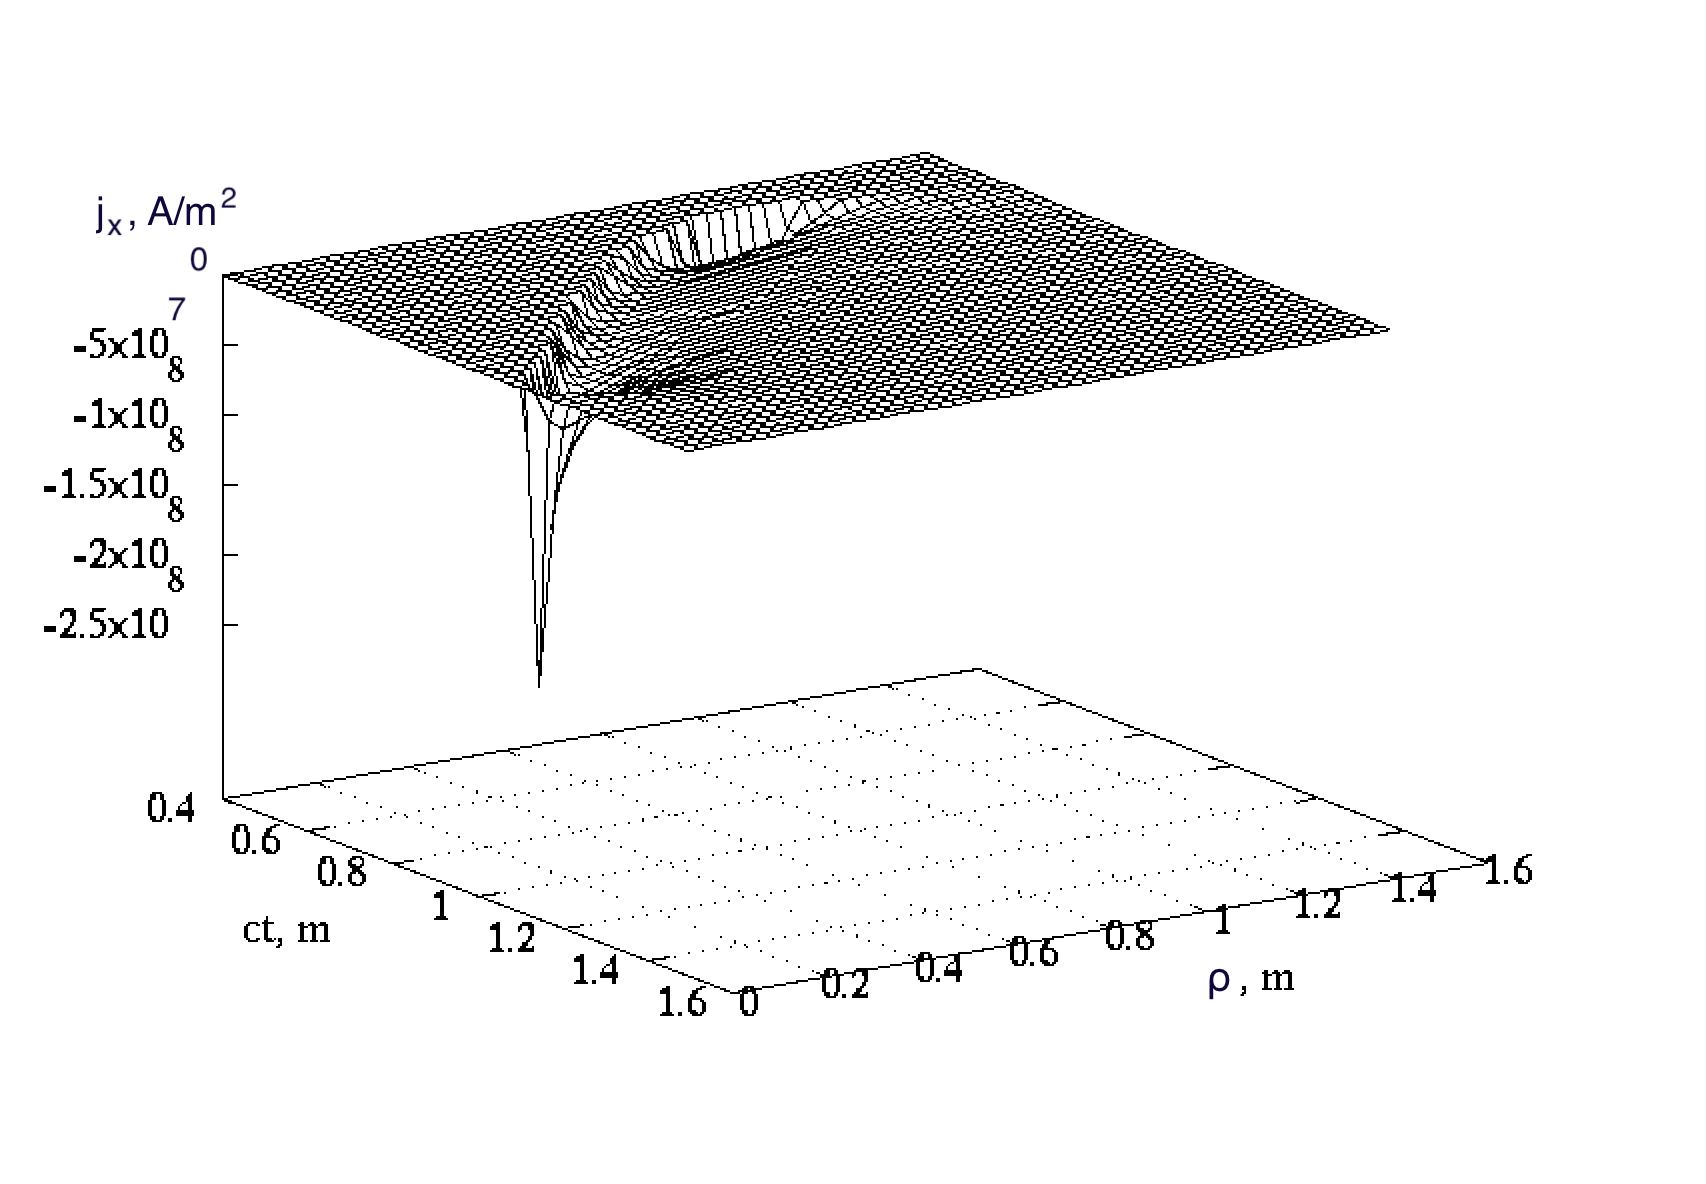
\includegraphics[width=5cm]{Jperp_A2} }}%
    \caption{Нелінійність амплітуди вторинного джерела}
    \label{fig:example}%
\end{figure}

Остання рівність складається з двох додаків. Перший додаток відповідає саме 
нелінійним властивостям поля. Останній додаток описує провідникові властивості 
середи розповлюдження, які теж мжуть бути описані вторинним джерелом. 
%
\begin{equation*} 
\vect{J^\prime} = 
\vect{\rho_0}    \partder{}{t} P_\rho^\prime    \left( \vect{E} \right) + 
\vect{\varphi_0} \partder{}{t} P_\varphi^\prime \left( \vect{E} \right) + 
\vect{z_0}       \partder{}{t} P_z^\prime       \left( \vect{E} \right) 
\end{equation*}
%
Вектор поляризвції для середовищі, де спостерігаюсься слабкі нелінійні ефкекти 
є довільною функцією, але може бути представлено в виді розкладу степеневого 
ряду Тейлора. 
%
\begin{equation*} \begin{aligned}
\vect{P^\prime} \left( \vect{E} \right) = \sum_{i=2}^{\infty} \xi_i \vect{E}^i
\end{aligned} \end{equation*}
%
Зауважимо, що розклад ведется по степеням вектора напружиності 
електричного поля, як у задачах оптики \textcolor{red}{[ПОСИЛАННЯ]}. 
Це створює математичні проблеми у доданках з парними коефіцієнтами.
вирішити їх можна домноженням на одиничний вектор.
%
\begin{equation*} \begin{aligned}
\vect{P^\prime}_2 \left( \vect{E} \right) = \xi_2 \vect{E}^2 = 
\xi_2 \vect{E}^2 \left( \vect{\rho_0}  + \vect{\varphi_0} + \vect{z_0} \right)
\end{aligned} \end{equation*}
%
\textcolor{red}{ Згідно з неоднозначностю векторного потенціалу 
\cite[ст. 77]{imp:LandauII} $ \vect{J^\prime} \left\{ S_1 \right\}  = 0 $. }
%
\textcolor{red}{ Чи правильно, що нелінійна ппроникність поля залежеть від 
амплтуди джерела? }
%
Для аналізу виберемо третій доданок неліної поляризації, який активно 
використовується в імпульсній електроніці \textcolor{red}{[ПОСИЛАННЯ]}.
%
\begin{equation*}
\vect{P^\prime} \left( \vect{E} \right) = 
\xi_3^e \vect{E}^3 
\left( A_0, R, \epsilon, \mu, vt, \vect{r} \right)
\end{equation*}
%
Під кубом вектора розуміється сам вектор домноженій на квадрат довжини.
\textcolor{red}{ Можливо, що природа нелінійних ефектів значно глибша і 
їх ефект впливає на характер енегетичної взаємодії та змінює простір.
Відповідно довжина вектора в декартовому сенсі втрачає змаст. }
%
\begin{equation*}
\vect{P^\prime} \left( \vect{E} \right) = 
\xi_3^e \dotprod{ \vect{E} }{ \vect{E} } \cdot \vect{E} 
\end{equation*}
%
В середовищі, де нелінійні ефекти описуються таким вектором
%
\textcolor{lightgray}{ \begin{equation*} \begin{aligned}
\vect{P^\prime} \left( \vect{E} \right) = 
\frac{ {A_0}^3 \xi_3^e }{ 8 } \left( \frac{\mu_0 \mu}
{\epsilon_0 \epsilon} \right)^{3/2} \left( {I_1}^2 \cos^2 \varphi + 
\left( I_2 - I_1 \right)^2 \sin^2 \varphi \right) \cdot \\ 
\cdot \Big( \vect{\rho_0} I_1 \cos \varphi - 
\vect{ \varphi_0 } \left( I_2 - I_1 \right) \sin \varphi \Big)
\end{aligned} \end{equation*} }
%
\textcolor{red}{ Які нелінійні ефекти спостерігаються в керрівському середовищі?}

%%%%%%%%%%%%%%%%%%%%%%%%%%%%%%%%%%%%%%%%%%%%%%%%%%%%%%%%%%%%%%%%%%%%%%%%%%%%%%%%
\section{Еволюційні коефіцієнти для нелінійної поправки до поля}
%
Для отримання нелінійної поправки до електричного поля спочатку отримаємо
розкладене по модовому базису вторинне джерело поля. Для цього, 
\textcolor{red}{згідно принципам віпромінювання}, знадобляться 
похідні компонентів електричного поля за часом. Часова залежність лінійного
електричного поля плаского дику міститься тільки в функціях 
$ I_1(ct,r) $ та $ I_2(ct,r) $. Для збереження безрозмарності розділимо
похідні на максимальну швидкість розповсюдженя для середовища.
%
\textcolor{lightgray}{ \begin{equation*} \begin{aligned}
I_1 \left\{ S_2 \right\} = \frac{\rho^2 + R^2}{4 \pi \rho^2} \arccos 
\frac{c^2 t^2 - z^2 - \rho^2 - R^2}{2 \rho R}  -
\frac{\sqrt{4 \rho^2 R^2 - (\rho^2 + R^2 - c^2t^2 + z^2)^2}}{4 \pi \rho^2} - \\
- \frac{ |\rho^2 - R^2| }{2 \pi \rho^2} 
\arctan \sqrt{ \frac{(\rho - R)^2}{(\rho + R)^2} \cdot
\frac{\left( \rho + R \right)^2 - \left( c^2t^2 - z^2 \right)} 
{\left( c^2t^2 - z^2 \right) - \left( \rho - R \right)^2} }
\end{aligned} \end{equation*} }
%
\textcolor{lightgray}{ \begin{equation*} \begin{aligned}
\partder{I_1 \left\{ S_2 \right\}}{t} = \frac{\rho^2 + R^2}{4 \pi \rho^2}
\partder{}{t} \arccos \frac{c^2 t^2 - z^2 - \rho^2 - R^2}{2 \rho R} - \\
- \partder{}{t} \frac{\sqrt{4 \rho^2 R^2 - (\rho^2 + R^2 - c^2t^2 + z^2)^2}}
{4 \pi \rho^2} - \\ - \frac{ |\rho^2 - R^2| }{2 \pi \rho^2} \partder{}{t} 
\arctan \sqrt{ \frac{(\rho - R)^2}{(\rho + R)^2} \cdot
\frac{\left( \rho + R \right)^2 - \left( c^2t^2 - z^2 \right)} 
{\left( c^2t^2 - z^2 \right) - \left( \rho - R \right)^2} }
\end{aligned} \end{equation*} }
%
\textcolor{lightgray}{ \begin{equation*} \begin{aligned}
\partder{}{t} \arccos \frac{c^2 t^2 - z^2 - \rho^2 - R^2}{2 \rho R} = 
- \frac{2 c^2 t}
{ \sqrt{4 \rho^2 R^2 - \left(c^2 t^2 - z^2 - \rho^2 - R^2 \right)^2} }
\end{aligned} \end{equation*} }
%
\textcolor{red}{ \begin{equation*} \begin{aligned}
- \partder{}{t} \left( \rho^2 + R^2 - c^2t^2 + z^2 \right)^2 = 
- 2 (\rho^2 + R^2 -c^2t^2 + z^2) (-2 c^2 t)
\end{aligned} \end{equation*} }
%
\textcolor{lightgray}{ \begin{equation*} \begin{aligned}
\partder{}{t} \frac{\sqrt{4 \rho^2 R^2 - (\rho^2 + R^2 - c^2t^2 + z^2)^2}}
{4 \pi \rho^2} = \frac{1}{8 \pi \rho^2} 
\frac{ 4 c^2 t (\rho^2 + R^2 - c^2 t^2 + z^2) }
{ \sqrt{4 \rho^2 R^2 - (\rho^2 + R^2 - c^2t^2 + z^2)^2} } = \\
= \frac{c^2 t}{2 \pi \rho^2} \frac{\rho^2 + R^2 - c^2 t^2 + z^2}
{ \sqrt{4 \rho^2 R^2 - (\rho^2 + R^2 - c^2t^2 + z^2)^2} }
\end{aligned} \end{equation*} }
%
\textcolor{red}{ \begin{equation*} \begin{aligned}
\partder{}{t} \arctan \sqrt{ \frac{x}{y} } = 
\frac{1}{1 + \frac{x}{y}} \frac{1}{2} 
\sqrt \frac{y}{x} \partder{}{t} \frac{x}{y}
\end{aligned} \end{equation*} }
%
\textcolor{red}{ \begin{equation*} \begin{aligned}
- \frac{1}{(\rho + R)^2} + \frac{1}{(\rho - R)^2} = 
\frac{- (\rho-R)^2 + (\rho+R)^2 }{ (\rho^2 - R^2)^2 }
\end{aligned} \end{equation*} }
%
\textcolor{lightgray}{ \begin{equation*} \begin{aligned}
\partder{}{t} \arctan \sqrt{ \frac{(\rho - R)^2}{(\rho + R)^2}
\frac{\left( \rho + R \right)^2 - \left( c^2t^2 - z^2 \right)} 
{\left( c^2t^2 - z^2 \right) - \left( \rho - R \right)^2} } = 
\partder{}{t} \arctan \sqrt{ \frac
{1 - \frac{c^2t^2 - z^2}{\left( \rho + R \right)^2} } 
{ \frac{c^2t^2 - z^2}{ \left( \rho - R \right)^2 } - 1} } = \\
= \frac{1}{1 + \frac{1 - \frac{c^2t^2 - z^2}{\left( \rho + R \right)^2} } 
{ \frac{c^2t^2 - z^2}{ \left( \rho - R \right)^2 } - 1} } \frac{1}{2}
\sqrt{ \frac{ \frac{c^2t^2 - z^2}{ \left( \rho - R \right)^2 } - 1 }
{1 - \frac{c^2t^2 - z^2}{\left( \rho + R \right)^2} } } 
\frac{ - \frac{2 c^2 t}{\left( \rho + R \right)^2} 
\left( \frac{c^2t^2 - z^2}{ \left( \rho - R \right)^2} - 1 \right) - 
\frac{ 2 c^2 t }{ \left( \rho - R \right)^2 } 
\left( 1 - \frac{c^2t^2 - z^2}{\left( \rho + R \right)^2} \right) }
{\left( \frac{c^2t^2 - z^2}{ \left( \rho - R \right)^2 } - 1 \right)^2} = \\
= - c^2 t \frac{ \frac{c^2t^2-z^2}{(\rho-R)^2} - 1 }
{ \frac{c^2t^2-z^2}{(\rho-R)^2} - 1 + 1 - 
\frac{c^2t^2 - z^2}{\left( \rho + R \right)^2} }
\sqrt{ \frac{ \frac{c^2t^2 - z^2}{ \left( \rho - R \right)^2 } - 1}
{1 - \frac{c^2t^2 - z^2}{\left( \rho + R \right)^2} } } \frac
{ \frac{c^2t^2 - z^2}{ \left( \rho^2 - R^2 \right)^2 } - \frac{1}{(\rho+R)^2} + 
\frac{1}{(\rho-R)^2} - \frac{ c^2t^2 - z^2 }{ \left( \rho^2 - R^2 \right)^2 } }
{ \left( \frac{c^2t^2 - z^2}{ \left( \rho - R \right)^2} - 1 \right)^2 } = \\
= - \frac{4 \rho R c^2 t}{ \left( \rho^2 - R^2 \right)^2 } 
\frac{ 1 }{ \frac{c^2t^2-z^2}{(\rho-R)^2} - 
\frac{c^2t^2 - z^2}{\left( \rho + R \right)^2} }
\sqrt{ \frac{ \frac{c^2t^2 - z^2}{ \left( \rho - R \right)^2 } - 1}
{1 - \frac{c^2t^2 - z^2}{\left( \rho + R \right)^2} } } \frac
{ 1 }{ \frac{c^2t^2 - z^2}{ \left( \rho - R \right)^2} - 1 } = \\
= - \frac{c^2 t}{ c^2 t^2 - z^2 } \frac{1} { 
\sqrt{ 1 - \frac{c^2t^2 - z^2}{(\rho + R)^2 } } 
\sqrt{ \frac{c^2t^2 - z^2}{ (\rho - R)^2 } - 1} }
\end{aligned} \end{equation*} }
%
\textcolor{lightgray}{ \begin{equation*} \begin{aligned}
\partder{ I_1 \{ S_2 \} }{t} = - \frac{c^2 t}{2 \pi \rho^2}
\frac{\rho^2 + R^2}
{ \sqrt{4 \rho^2 R^2 - \left(c^2 t^2 - z^2 - \rho^2 - R^2 \right)^2} } - \\
- \frac{c^2 t}{2 \pi \rho^2} \frac{\rho^2 + R^2 - c^2 t^2 + z^2}
{ \sqrt{4 \rho^2 R^2 - (\rho^2 + R^2 - c^2t^2 + z^2)^2} } + \\ 
+ \frac{ c^2 t }{2 \pi \rho^2} \frac{|\rho^2 - R^2|}{ c^2 t^2 - z^2 } \frac{1} 
{ \sqrt{ 1 - \frac{c^2t^2 - z^2}{(\rho + R)^2 } } 
\sqrt{ \frac{c^2t^2 - z^2}{ (\rho - R)^2 } - 1} }
\end{aligned} \end{equation*} }
%
\begin{equation*} \begin{aligned}
\frac{1}{c} \partder{ I_1 \{ S_2 \} }{t} = \frac{ ct }{2 \pi \rho^2} 
\frac{ (\rho^2 - R^2)^2  (c^2 t^2 - z^2)^{-1} } 
{ \sqrt{ (\rho + R)^2 - c^2t^2 + z^2 } 
\sqrt{ c^2t^2 - z^2 - (\rho - R)^2 } } - \\
- \frac{ct}{2 \pi \rho^2} \frac{2 (\rho^2 + R^2) - (c^2 t^2 - z^2)}
{ \sqrt{4 \rho^2 R^2 - (c^2t^2 - z^2 - \rho^2 - R^2)^2} }
\end{aligned} \end{equation*}
%
\begin{equation*} \begin{aligned}
\frac{1}{c} \partder{ I_1 \{ S_{1,3} \} }{t} = 0
\end{aligned} \end{equation*}
%
\textcolor{lightgray}{ \begin{equation*} \begin{aligned}
\partder{ I_2 \{ S_2 \} }{t} = \frac{1}{\pi} \partder{}{t} \arccos 
\frac{c^2t^2 - z^2 + \rho^2 - R^2}{2 \rho \sqrt{c^2t^2 - z^2}} = \\
= - \frac{1}{\pi} \frac{1} { \sqrt{ 1 - \frac{ (c^2t^2 - z^2 + \rho^2 - R^2)^2 }
{4 \rho^2 (c^2t^2 - z^2)^2} } } \frac{1}{2 \rho} \partder{}{t} 
\frac{c^2t^2 - z^2 + \rho^2 - R^2} {\sqrt{c^2t^2 - z^2}} = \\
= - \frac{1}{2 \rho \pi} \frac{1} 
{ \sqrt{ 1 - \frac{ (c^2t^2 - z^2 + \rho^2 - R^2)^2 }
{4 \rho^2 (c^2t^2 - z^2)} } } \frac{2c^2t \sqrt{c^2t^2 - z^2} - 
\frac{c^2t}{\sqrt{c^2t^2 - z^2}} (c^2t^2 - z^2 + \rho^2 - R^2)
}{c^2t^2 - z^2} = \\ = - \frac{c^2 t}{2 \pi \rho} \frac{1} 
{ \sqrt{ 1 - \frac{ (c^2t^2 - z^2 + \rho^2 - R^2)^2 }
{4 \rho^2 (c^2t^2 - z^2)} } } \frac{2 \sqrt{c^2t^2 - z^2} - 
\frac{c^2t^2 - z^2 + \rho^2 - R^2}{\sqrt{c^2t^2 - z^2}}}{c^2t^2 - z^2} = \\
= - \frac{c^2 t}{2 \pi \rho (c^2t^2 - z^2)} \frac{ 2 \sqrt{c^2t^2 - z^2} - 
\frac{c^2t^2 - z^2 + \rho^2 - R^2}{\sqrt{c^2t^2 - z^2}} } 
{ \sqrt{ 1 - \frac{ (c^2t^2 - z^2 + \rho^2 - R^2)^2 }
{4 \rho^2 (c^2t^2 - z^2)} } } = \\
= - \frac{c^2 t}{\pi (c^2t^2 - z^2) } 
\frac{ 2 (c^2t^2 - z^2) - (c^2t^2 - z^2 + \rho^2 - R^2) } 
{ \sqrt{ 4 \rho^2 (c^2t^2 - z^2) - (c^2t^2 - z^2 + \rho^2 - R^2)^2 } } = \\
= - \frac{c^2 t}{\pi (c^2t^2 - z^2) } \frac{ c^2t^2 - z^2 -  \rho^2 + R^2 } 
{ \sqrt{ 4 \rho^2 (c^2t^2 - z^2) - (c^2t^2 - z^2 + \rho^2 - R^2)^2 } }
\end{aligned} \end{equation*} }
%
\begin{equation*} \begin{aligned}
\frac{1}{c} \partder{ I_2 \{ S_2 \} }{t} = 
- \frac{ct}{\pi (c^2t^2 - z^2) } \frac{ c^2t^2 - z^2 -  \rho^2 + R^2 } 
{ \sqrt{ 4 \rho^2 (c^2t^2 - z^2) - (c^2t^2 - z^2 + \rho^2 - R^2)^2 } }
\end{aligned} \end{equation*}
%
\begin{equation*} \begin{aligned}
\frac{1}{c} \partder{ I_2 \{ S_{1,3} \} }{t} = 0
\end{aligned} \end{equation*}
%
Як було показано раніше, область значень $ I_1 $ та $ I_2 $ визначається 
просторовими змінними та часом, отже похідні $ \partder{I_1}{t} $ та 
$ \partder{I_1}{t} $ треба брати з урахуванням областей $ S_1 $, $ S_2 $ та
$ S_3 $.
%
\begin{equation*} \begin{aligned}
\partder{I_\alpha}{\tau} = \partder{ I_k \{ S_{2} \} }{\tau} \Big( 
H \left( \tau^2 - z^2 - (\rho - R)^2 \right)  - 
H \left( \tau^2 - z^2 - (\rho + R)^2 \right) \Big) + \\
+ 2 \tau I_\alpha \{ S_{2} \} \Big( 
\delta \left( \tau^2 - z^2 - (\rho - R)^2 \right)  - 
\delta \left( \tau^2 - z^2 - (\rho + R)^2 \right) \Big) + \\
+ \frac{2 \tau}{\alpha} \delta \left( \tau^2 - z^2 - (\rho + R)^2 \right)
\end{aligned} \end{equation*}
%
Підставляючи $ I_\alpha \{ S_{2} \} $ до останього виразу бачимо, що другий доданок знакає.
%
\begin{equation*} \begin{aligned}
\partder{I_\alpha}{\tau} = \frac{2 \tau}{\alpha} 
\delta \left( \tau^2 - z^2 - (\rho + R)^2 \right) + \\
+ \partder{ I_k \{ S_{2} \} }{\tau} \Big( 
H \left( \tau^2 - z^2 - (\rho - R)^2 \right)  - 
H \left( \tau^2 - z^2 - (\rho + R)^2 \right) \Big)
\end{aligned} \end{equation*}
%
Тепер запишемо компоненти електричного струму, який є вторинним джерелом
електромагнітного поля. З компонентою $ \vect{z_0} $ все просто - 
поздовжне електричне поле дорівнює нулю.
%
\textcolor{lightgray}{ \begin{equation*} \begin{aligned}
\vect{P^\prime} \left( \vect{E} \right) = 
\frac{ {A_0}^3 \xi_3 }{ 8 } \left( \frac{\mu_0 \mu}
{\epsilon_0 \epsilon} \right)^{3/2} \left( {I_1}^2 \cos^2 \varphi + 
\left( I_2 - I_1 \right)^2 \sin^2 \varphi \right) \cdot \\ 
\cdot \Big( \vect{\rho_0} I_1 \cos \varphi - 
\vect{ \varphi_0 } \left( I_2 - I_1 \right) \sin \varphi \Big)
\end{aligned} \end{equation*} }
%
\textcolor{lightgray}{ \begin{equation*} \label{eq:linear_e_cyl}
\vect{E} = \frac{A_0}{2} \sqrt{\frac{\mu_0 \mu}{\epsilon_0 \epsilon}}
\Big( \vect{\rho_0} I_1 \cos \varphi - 
\vect{ \varphi_0 } \left( I_2 - I_1 \right) \sin \varphi \Big)
\end{equation*} }
%
\textcolor{lightgray}{ \begin{equation*} \begin{aligned}
\vect{E}^2 = \frac{A_0^2}{4} \frac{\mu_0 \mu}{\epsilon_0 \epsilon}
\Big( I_1^2 \cos^2 \varphi + \left( I_2 - I_1 \right)^2 \sin^2 \varphi \Big)
\end{aligned} \end{equation*} }
%
\textcolor{lightgray}{ \begin{equation*} \begin{aligned}
\partder{ \vect{E}^2 }{t} = \frac{A_0^2}{4} 
\frac{\mu_0 \mu}{\epsilon_0 \epsilon}
\left( 2 I_1 \partder{I_1}{t} \cos^2 \varphi + 
2 ( I_2 - I_1 ) \left( \partder{I_2}{t} - \partder{I_1}{t} \right) 
\sin^2 \varphi \right)
\end{aligned} \end{equation*} }
%
\begin{equation*} \begin{aligned}
\partder{P_z^\prim}{t} = 0
\end{aligned} \end{equation*}
%
Вирази для поперечних компонентів поля стають шматочновизначиними,
через свої залежності.
%
\textcolor{lightgray} { \begin{equation*} \begin{aligned}
\partder{P_\rho^\prime}{t}   = \frac{ {A_0}^3 \xi_3 }{ 8 } 
\left( \frac{\mu_0 \mu} {\epsilon_0 \epsilon} \right)^{3/2} \left(
\left( {I_1}^2 \cos^2 \varphi + ( I_2 - I_1 )^2 \sin^2 \varphi \right)
\partder{I_1}{t} \cos \varphi + \right. \\
\left. + I_1 \cos \varphi \left( 2 I_1 \partder{I_1}{t} \cos^2 \varphi + 
2 ( I_2 - I_1 ) \left( \partder{I_2}{t} - \partder{I_1}{t} \right) 
\sin^2 \varphi \right) \right) = \\ = \frac{ {A_0}^3 \xi_3^e }{ 8 } 
\left( \frac{\mu_0 \mu} {\epsilon_0 \epsilon} \right)^{3/2} \left(
\partder{I_1}{t} {I_1}^2 \cos^3 \varphi + \partder{I_1}{t} ( I_2 - I_1 )^2 
\cos \varphi \sin^2 \varphi + \right. \\
\left. + 2 {I_1}^2 \partder{I_1}{t} \cos^3 \varphi + 
2 I_1 ( I_2 - I_1 ) \left( \partder{I_2}{t} - \partder{I_1}{t} \right) 
\cos \varphi \sin^2 \varphi \right)
\end{aligned} \end{equation*} }
%
\begin{equation*} \begin{aligned}
\partder{P_\rho^\prime}{t} = \frac{ {A_0}^3 \xi_3 }{ 8 } 
\left( \frac{\mu_0 \mu} {\epsilon_0 \epsilon} \right)^{3/2} \left(
3 {I_1}^2 \partder{I_1}{t} \cos^3 \varphi + \right. \\
+ \left. ( I_2 - I_1 ) \cos \varphi \sin^2 \varphi \left( 
\partder{I_1}{t} ( I_2 - I_1 ) + 2 I_1 \left( \partder{I_2}{t} - 
\partder{I_1}{t} \right) \right) \right)
\end{aligned} \end{equation*}
%
\textcolor{lightgray} { \begin{equation*} \begin{aligned}
\partder{P_\varphi^\prime}{t}   = - \frac{ {A_0}^3 \xi_3 }{ 8 } 
\left( \frac{\mu_0 \mu} {\epsilon_0 \epsilon} \right)^{3/2} \left(
\left( {I_1}^2 \cos^2 \varphi + ( I_2 - I_1 )^2 \sin^2 \varphi \right)
\left( \partder{I_2}{t} - \partder{I_1}{t} \right) \sin \varphi + \right. \\
\left. + (I_2 - I_1) \sin \varphi \left( 2 I_1 \partder{I_1}{t} \cos^2 \varphi + 
2 ( I_2 - I_1 ) \left( \partder{I_2}{t} - \partder{I_1}{t} \right) 
\sin^2 \varphi \right) \right) = \\ = - \frac{ {A_0}^3 \xi_3 }{ 8 } 
\left( \frac{\mu_0 \mu} {\epsilon_0 \epsilon} \right)^{3/2} \left(
{I_1}^2 \left( \partder{I_2}{t} - \partder{I_1}{t} \right) 
\sin \varphi \cos^2 \varphi + \right. \\ \left. 
+ ( I_2 - I_1 )^2 \left( \partder{I_2}{t} - \partder{I_1}{t} \right) 
\sin^3 \varphi + 2 I_1 \partder{I_1}{t} (I_2 - I_1) 
\sin \varphi \cos^2 \varphi + \right. \\ 
+ \left. 2 ( I_2 - I_1 )^2 \left( \partder{I_2}{t} - \partder{I_1}{t} \right) 
\sin^3 \varphi \right)
\end{aligned} \end{equation*} }
%
\begin{equation*} \begin{aligned}
\partder{P_\varphi^\prime}{t} = - \frac{ {A_0}^3 \xi_3 }{ 8 } 
\left( \frac{\mu_0 \mu} {\epsilon_0 \epsilon} \right)^{3/2} \left(
3 ( I_2 - I_1 )^2 \left( \partder{I_2}{t} - \partder{I_1}{t} \right)
\sin^3 \varphi \right. + \\
+ \left. I_1 \sin \varphi \cos^2 \varphi \left( 
I_1 \left( \partder{I_2}{t} - \partder{I_1}{t} \right) + 
2 \partder{I_1}{t} (I_2 - I_1) \right) \right)
\end{aligned} \end{equation*}
%
Для запису модового струму використаємо формулу ..., що 
є кратиним інтегралом по точкам випромінювання та має комплексну
область значень.
%
\textcolor{lightgray} { \begin{equation*}
j_m \left( r, t; \nu \right) = \frac{\sqrt{\mu_0}}{2\pi} 
\int \limits_{0}^{2\pi} d \varphi \int \limits_0^\infty \rho d \rho 
\vect{j_0} \crossprod{ \nabla_\perp \Psi_m^* }{ \vect{z_0} }
\end{equation*} }
%
\textcolor{lightgray} { \begin{equation*} 
\vect{J^\prime} = 
\vect{\rho_0}    \partder{}{t} P_\rho^\prime    \left( \vect{E} \right) + 
\vect{\varphi_0} \partder{}{t} P_\varphi^\prime \left( \vect{E} \right) + 
\vect{z_0}       \partder{}{t} P_z^\prime       \left( \vect{E} \right) 
\end{equation*} }
%
\textcolor{lightgray} { \begin{equation*} \begin{aligned}
\crossprod{ \nabla_\perp \Psi_m^* }{ \vect{z_0} } =
- \vect{\rho_0} i m e^{-im\varphi} \frac{J_m (\nu \rho)}{\rho \sqrt{\nu}}
- \vect{\varphi_0} \sqrt{\nu} e^{-im\varphi} 
\frac{J_{m-1} (\nu \rho) - J_{m+1} (\nu \rho)}{2}
\end{aligned} \end{equation*} }
%
\textcolor{lightgray} { \begin{equation*} \begin{aligned}
\vect{J^\prime} \crossprod{ \nabla_\perp \Psi_m^* }{ \vect{z_0} } = 
- i e^{-im\varphi} m \frac{J_m (\nu \rho)}{\rho \sqrt{\nu}}
\partder{}{t} P_\rho^\prime \left( \vect{E} \right) - \\
- \sqrt{\nu} e^{-im\varphi} \frac{J_{m-1} (\nu \rho) - J_{m+1} (\nu \rho)}{2}
\partder{}{t} P_\varphi^\prime \right)
\end{aligned} \end{equation*} }
%
\begin{equation*} \begin{aligned}
j_m = - \frac{\sqrt{\mu_0}}{2\pi} 
\int_{0}^{2\pi} d \varphi \int \limits_{0}^{\infty} \rho d \rho
e^{-im\varphi} \left( i  m \frac{J_m (\nu \rho)}{\rho \sqrt{\nu}}
\partder{P_\rho^\prime}{t} + \sqrt{\nu}
\frac{J_{m-1} (\nu \rho) - J_{m+1} (\nu \rho)}{2}
\partder{P_\varphi^\prime}{t} \right)
\end{aligned} \end{equation*}
%
Згрупувавши доданки за тригонометричними функціями, що вони містять,
знайдемо інтеграли за зменним азимутальним кутом $ \varphi $. Самі інеграли
взяті окремо в додатку ..., випишимо лише результати.
%
\textcolor{lightgray} { \begin{equation*} \begin{aligned}
\int_{0}^{2 \pi} d \varphi e^{-im \varphi} \partder{P_\rho^\prime}{t} = 
\frac{ {A_0}^3 \xi_3 }{ 8 } \int_{0}^{2\pi} d \varphi
e^{-im\varphi} \left( \frac{\mu_0 \mu} {\epsilon_0 \epsilon} \right)^{3/2} 
\left( 3 {I_1}^2 \partder{I_1}{t} \cos^3 \varphi + \right. \\
+ \left. ( I_2 - I_1 ) \cos \varphi \sin^2 \varphi \left( 
\partder{I_1}{t} ( I_2 - I_1 ) + 2 I_1 \left( \partder{I_2}{t} - 
\partder{I_1}{t} \right) \right) \right) = \\
= \frac{ {A_0}^3 \xi_3 }{ 8 } 
\left( \frac{\mu_0 \mu} {\epsilon_0 \epsilon} \right)^{3/2}
\left( \frac{3 \pi}{4} {I_1}^2 \partder{I_1}{t} \left( \delta_{m,-3} - 
\delta_{m,3} + 3 \delta_{m,-1} + 3 \delta_{m,1} \right) + \right. \\
+ \frac{\pi }{4} \left. ( I_2 - I_1 ) \left( \delta_{m,1} - 
\delta_{m,-3} + \delta_{m,-1} - \delta_{m,3} \right) \left( 
\partder{I_1}{t} ( I_2 - I_1 ) + 2 I_1 \left( \partder{I_2}{t} - 
\partder{I_1}{t} \right) \right) \right)
\end{aligned} \end{equation*} }
%
\textcolor{lightgray} { \begin{equation*} \begin{aligned}
\int_{0}^{2\pi} e^{-i m \varphi} \cos^3 \varphi d \varphi = 
\frac{\pi}{4} \delta_{m,-3} - \frac{\pi}{4} \delta_{m,3} + 
\frac{3 \pi}{4} \delta_{m,-1} + \frac{3 \pi}{4} \delta_{m,1}
\end{aligned} \end{equation*} }
%
\textcolor{lightgray} { \begin{equation*} \begin{aligned}
\int_{0}^{2\pi} e^{-i m \varphi} \cos \varphi \sin^2 \varphi d \varphi = 
\frac{\pi \delta_{m,1} }{4} - \frac{\pi \delta_{m,-3} }{4} + 
\frac{\pi \delta_{m,-1} }{4} - \frac{\pi \delta_{m,3} }{4}
\end{aligned} \end{equation*} }
%
\begin{equation*} \begin{aligned}
\int_{0}^{2\pi} d \varphi e^{-im \varphi} \partder{P_\rho^\prime}{t} = 
\frac{ {A_0}^3 \xi_3 \pi }{ 4 \cdot 8 } 
\left( \frac{\mu_0 \mu} {\epsilon_0 \epsilon} \right)^{3/2}
\left( 3 {I_1}^2 \partder{I_1}{t} \left( \delta_{m,-3} - 
\delta_{m,3} + 3 \delta_{m,-1} + 3 \delta_{m,1} \right) + \right. \\
+ \left. ( I_2 - I_1 ) \left( \delta_{m,1} - 
\delta_{m,-3} + \delta_{m,-1} - \delta_{m,3} \right) \left( 
\partder{I_1}{t} ( I_2 - I_1 ) + 2 I_1 \left( \partder{I_2}{t} - 
\partder{I_1}{t} \right) \right) \right)
\end{aligned} \end{equation*}
%
\textcolor{lightgray} { \begin{equation*} \begin{aligned}
\int_{0}^{2\pi} e^{-i m \varphi} \sin^3 \varphi d \varphi = 
\frac{3 \pi i}{4} \delta_{m,-1} - \frac{3 \pi i}{4} \delta_{m,1} - 
\frac{\pi i}{4} \delta_{m,-3} - \frac{\pi i}{4} \delta_{m,3}
\end{aligned} \end{equation*} }
%
\textcolor{lightgray} { \begin{equation*} \begin{aligned}
\int_{0}^{2\pi} e^{-i m \varphi} \sin \varphi \cos^2 \varphi d \varphi = 
\frac{\pi i }{4} \delta_{m,-3} - \frac{\pi i }{4} \delta_{m,1} + 
\frac{\pi i }{4} \delta_{m,3} + \frac{\pi i }{4} \delta_{m,-1}
\end{aligned} \end{equation*} }
%
\textcolor{lightgray} { \begin{equation*} \begin{aligned}
\int_{0}^{2 \pi} d \varphi e^{-im \varphi} \partder{P_\varphi^\prime}{t} = \\
= - \frac{ {A_0}^3 \xi_3 }{ 8 } \int_{0}^{2 \pi} d \varphi e^{-im \varphi}
\left( \frac{\mu_0 \mu} {\epsilon_0 \epsilon} \right)^{3/2} \left(
3 ( I_2 - I_1 )^2 \left( \partder{I_2}{t} - \partder{I_1}{t} \right)
\sin^3 \varphi \right. + \\
+ \left. I_1 \sin \varphi \cos^2 \varphi \left( 
I_1 \left( \partder{I_2}{t} - \partder{I_1}{t} \right) + 
2 \partder{I_1}{t} (I_2 - I_1) \right) \right) = 
- \frac{ {A_0}^3 \xi_3 }{ 8 V } \cdot \\ 
\cdot \left( \frac{\mu_0 \mu} {\epsilon_0 \epsilon} \right)^{3/2} \left(
\frac{3 \pi i}{4} ( I_2 - I_1 )^2 \left( \partder{I_2}{t} - 
\partder{I_1}{t} \right) \left( 3 \delta_{m,-1} - 3 \delta_{m,1} - 
\delta_{m,-3} - \delta_{m,3} \right) \right. + \\
+ \left. \frac{\pi i}{4} I_1 \left(  \delta_{m,-3} - \delta_{m,1} + 
\delta_{m,3} + \delta_{m,-1} \right) \left( 
I_1 \left( \partder{I_2}{t} - \partder{I_1}{t} \right) + 
2 \partder{I_1}{t} (I_2 - I_1) \right) \right)
\end{aligned} \end{equation*} }
%
\begin{equation*} \begin{aligned}
\int_{0}^{2 \pi} d \varphi e^{-im \varphi} \partder{P_\varphi^\prime}{t} = 
- \frac{ {A_0}^3 \xi_3  i \pi }{ 4 \cdot 8 }
\left( \frac{\mu_0 \mu} {\epsilon_0 \epsilon} \right)^{3/2} \cdot \\ 
\cdot \left( 3 ( I_2 - I_1 )^2 \left( \partder{I_2}{t} - 
\partder{I_1}{t} \right) \left( 3 \delta_{m,-1} - 3 \delta_{m,1} - 
\delta_{m,-3} - \delta_{m,3} \right) \right. + \\
+ \left. I_1 \left(  \delta_{m,-3} - \delta_{m,1} + 
\delta_{m,3} + \delta_{m,-1} \right) \left( 
I_1 \left( \partder{I_2}{t} - \partder{I_1}{t} \right) + 
2 \partder{I_1}{t} (I_2 - I_1) \right) \right)
\end{aligned} \end{equation*}
%
\textcolor{lightgray} { \begin{equation*} \begin{aligned}
\int \limits_{0}^{2\pi} d \varphi \sin \varphi 
\left( \cos m \varphi - i \sin m \varphi \right) = 
i \pi \left( \delta_{m,-1} - \delta_{m,1} \right)
\end{aligned} \end{equation*} }
%
\textcolor{lightgray} { \begin{equation*} \begin{aligned}
\int \limits_{0}^{2\pi} d \varphi \cos \varphi 
( \cos m \varphi - i \sin m \varphi) = \pi ( \delta_{m,-1} + \delta_{m,1} )
\end{aligned} \end{equation*} }
%
Тепер введемо нові змінні для того, щоб записати струм в визначенні модового 
базису, як інтеграл за радиалькою координатою $ \rho $. Тут з'являються змінні
за штрихованими кординатами. Так ми означимо кординати джерела випромінювання,
щоб уникнути плутанини з кординатами точки спостереження. Нехай ...
%
\textcolor{lightgray} { \begin{equation*} \begin{aligned}
N_1 (m) =  \frac{3 m {A_0}^3 \xi_3 \sqrt{\mu_0}}{64 \sqrt{\nu}} \frac{\pi}{\pi}
\left( \frac{\mu_0 \mu} {\epsilon_0 \epsilon} \right)^{3/2} 
\int_{0}^{\infty} d \rho 
J_m (\nu \rho) {I_1}^2 \partder{I_1}{t}
\end{aligned} \end{equation*} }
%
\textcolor{lightgray} { \begin{equation*} \begin{aligned}
N_1 (m) =  3 m J_m (\nu \rho) {I_1}^2 \partder{I_1}{t}
\end{aligned} \end{equation*} }
%
\begin{equation*} \begin{aligned}
N_1 (m) =  3 m J_m (\nu \rho') {I_1}^2 \partder{I_1}{t'}
\end{aligned} \end{equation*}
%
\textcolor{lightgray} { \begin{equation*} \begin{aligned}
N_1 (m) =  3 m J_m (\nu \rho') \begin{cases}
0^2 \cdot 2 \tau' \delta_+ \\
{f_1}^2 \left( \partder{f_1}{t'} + 2 \tau' \delta_+ \right) \\
1^2 \cdot 2 \tau' \delta_+
\end{cases} \end{aligned} \end{equation*} }
%
\textcolor{lightgray} { \begin{equation*} \begin{aligned}
N_1 (m) =  3 m J_m (\nu \rho') \begin{cases} 0 \\
2 \tau' \delta_+ {f_1}^2 + \partder{f_1}{t'} {f_1}^2 \\
2 \tau' \delta_+
\end{cases} \end{aligned} \end{equation*} }
%
\begin{equation*} \begin{aligned}
N_1^\delta (m) = 3 m {I_1}^2 J_m (\nu \rho')
\end{aligned} \end{equation*}
%
\begin{equation*} \begin{aligned}
N_1^* (m) =  3 m J_m (\nu \rho') {I_1}^2 \partder{I_1}{t'}
\end{aligned} \end{equation*}
%
\textcolor{lightgray} { \begin{equation*} \begin{aligned}
N_2 (m) = \frac{m {A_0}^3 \xi_3 \sqrt{\mu_0}}{64 \sqrt{\nu}} \frac{\pi}{\pi}
\left( \frac{\mu_0 \mu} {\epsilon_0 \epsilon} \right)^{3/2} 
\int_{0}^{\infty} d \rho \\
J_m (\nu \rho) (I_2 - I_1) \left( \partder{I_1}{t} (I_2 - I_1) + 
2 I_1 \left( \partder{I_2}{t} - \partder{I_1}{t} \right) \right)
\end{aligned} \end{equation*} }
%
\textcolor{lightgray} { \begin{equation*} \begin{aligned}
N_2 (m) = m J_m (\nu \rho) (I_2 - I_1) \left( \partder{I_1}{t} (I_2 - I_1) + 
2 I_1 \left( \partder{I_2}{t} - \partder{I_1}{t} \right) \right)
\end{aligned} \end{equation*} }
%
\begin{equation*} \begin{aligned}
N_2 (m) = m J_m (\nu \rho') (I_2 - I_1) \left( \partder{I_1}{t'} (I_2 - I_1) + 
2 I_1 \left( \partder{I_2}{t'} - \partder{I_1}{t'} \right) \right)
\end{aligned} \end{equation*}
%
\textcolor{lightgray} { \begin{equation*} \begin{aligned}
N_2 (m) = m J_m (\nu \rho') \begin{cases}
2 \tau' \delta_+ (0 - 0)^2 + 0 (0 - 0) (2 \tau' \delta_+ - 2 \tau' \delta_+) \\
(f_2 - f_1)^2 (\partder{f_1}{t'} + 2 \tau' \delta_+) + 2 f_1 (f_2 - f_1) \left( 
\partder{f_2}{t'} - \partder{f_1}{t'} \right) \\
2 \tau' \delta_+ (0.5 - 1)^2 + 1 (0.5 - 1) (2 \tau' \delta_+ - 2 \tau' \delta_+)
\end{cases} \end{aligned} \end{equation*} }
%
\textcolor{lightgray} { \begin{equation*} \begin{aligned}
N_2 (m) = m J_m (\nu \rho') \begin{cases} 0 \\
2 \tau' \delta_+ (f_2 - f_1)^2 + (f_2 - f_1) 
\left( 2 f_1 \left( \partder{f_2}{t'} - \partder{f_1}{t'} \right) +
(f_2 - f_1) \partder{f_1}{t'} \right) \\
\tau' \delta_+ / 2
\end{cases} \end{aligned} \end{equation*} }
%
\begin{equation*} \begin{aligned}
N_2^\delta (m) = m J_m (\nu \rho') (I_2 - I_1)^2 
\end{aligned} \end{equation*}
%
\begin{equation*} \begin{aligned}
N_2^* (m) = m J_m (\nu \rho') (I_2 - I_1) \left( \partder{I_1}{t'} (I_2 - I_1) + 
2 I_1 \left( \partder{I_2}{t'} - \partder{I_1}{t'} \right) \right)
\end{aligned} \end{equation*}
%
\textcolor{lightgray} { \begin{equation*} \begin{aligned}
N_3 (m) = - \frac{3 {A_0}^3 \xi_3 \sqrt{\mu_0}}{64} \sqrt{\nu} \frac{\pi}{\pi}
\left( \frac{\mu_0 \mu} {\epsilon_0 \epsilon} \right)^{3/2} 
\int_{0}^{\infty} \rho d \rho 
\frac{J_{m-1} (\nu \rho) - J_{m+1} (\nu \rho)}{2} \\
(I_2 - I_1)^2 \left( \partder{I_2}{t} - \partder{I_1}{t} \right) 
\end{aligned} \end{equation*} }
%
\textcolor{lightgray} { \begin{equation*} \begin{aligned}
N_3 (m) = - 3 \nu \rho
\frac{J_{m-1} (\nu \rho) - J_{m+1} (\nu \rho)}{2}
(I_2 - I_1)^2 \left( \partder{I_2}{t} - \partder{I_1}{t} \right)
\end{aligned} \end{equation*} }
%
\begin{equation*} \begin{aligned}
N_3 (m) = - 3 \nu \rho'
\frac{J_{m-1} (\nu \rho') - J_{m+1} (\nu \rho')}{2}
(I_2 - I_1)^2 \left( \partder{I_2}{t'} - \partder{I_1}{t'} \right)
\end{aligned} \end{equation*}
%
\textcolor{lightgray} { \begin{equation*} \begin{aligned}
N_3 (m) = - 3 \nu \rho'
\frac{J_{m-1} (\nu \rho') - J_{m+1} (\nu \rho')}{2} \begin{cases}
(0-0)^2 (0 + 2 \tau' \delta_+ - 0 - 2 \tau' \delta_+) \\
(f_2 - f_1)^2 \left( \partder{f_2}{t'} - \partder{f_1}{t'} \right) \\
(0.5 - 1)^2 (0 + 2 \tau' \delta_+ - 0 - 2 \tau' \delta_+)
\end{cases} \end{aligned} \end{equation*} }
%
\textcolor{lightgray} { \begin{equation*} \begin{aligned}
N_3 (m) = - 3 \nu \rho'
\frac{J_{m-1} (\nu \rho') - J_{m+1} (\nu \rho')}{2} \begin{cases} 0 \\
(f_2 - f_1)^2 \left( \partder{f_2}{t'} - \partder{f_1}{t'} \right) \\ 0
\end{cases} \end{aligned} \end{equation*} }
%
\textcolor{lightgray} { \begin{equation*} \begin{aligned}
N_3 (m) = - 3 \nu \rho'
\frac{J_{m-1} (\nu \rho') - J_{m+1} (\nu \rho')}{2} \begin{cases} 0 \\
(f_2 - f_1)^2 \left( \partder{f_2}{t'} - \partder{f_1}{t'} \right) \\ 0
\end{cases} \end{aligned} \end{equation*} }
%
\begin{equation*} \begin{aligned}
N_3^\delta (m) = - 3 \nu \rho'
\frac{J_{m-1} (\nu \rho') - J_{m+1} (\nu \rho')}{2}
(I_2 - I_1)^2 \left( \partder{I_2}{t'} - \partder{I_1}{t'} \right)
\end{aligned} \end{equation*}
%
\begin{equation*} \begin{aligned}
N_3^* (m) = 0
\end{aligned} \end{equation*}
%
\textcolor{lightgray} { \begin{equation*} \begin{aligned}
N_4 (m) = - \frac{ {A_0}^3 \xi_3 \sqrt{\mu_0}}{64} \sqrt{\nu} \frac{\pi}{\pi}
\left( \frac{\mu_0 \mu} {\epsilon_0 \epsilon} \right)^{3/2}
\int_{0}^{\infty} \rho d \rho 
\frac{J_{m-1} (\nu \rho) - J_{m+1} (\nu \rho)}{2} \\
I_1 \left( I_1 \left( \partder{I_2}{t} - \partder{I_1}{t} \right) + 
2 \partder{I_1}{t} \left( I_2 - I_1 \right) \right)
\end{aligned} \end{equation*} }
%
\textcolor{lightgray} { \begin{equation*} \begin{aligned}
N_4 (m) = - \nu \rho
\frac{J_{m-1} (\nu \rho) - J_{m+1} (\nu \rho)}{2}
\left( I_1 \left( \partder{I_2}{t} - \partder{I_1}{t} \right) + 
2 \partder{I_1}{t} \left( I_2 - I_1 \right) \right)
\end{aligned} \end{equation*} }
%
\begin{equation*} \begin{aligned}
N_4 (m) = - \nu \rho'
\frac{J_{m-1} (\nu \rho') - J_{m+1} (\nu \rho')}{2} I_1
\left( I_1 \left( \partder{I_2}{t'} - \partder{I_1}{t'} \right) + 
2 \partder{I_1}{t'} \left( I_2 - I_1 \right) \right)
\end{aligned} \end{equation*}
%
\textcolor{lightgray} { \begin{equation*} \begin{aligned}
N_4 (m) \{ S_2 \} = {f_1}^2 
\left( \partder{f_2}{t'} - \partder{f_1}{t'} \right) + 
2 f_1 \left( \partder{f_1}{t'} + 2 \tau' \delta_+ \right) 
\left( f_2 - f_1 \right) = \\
= f_1^2 \left( \partder{f_2}{t'} - 3 \partder{f_1}{t'} \right) 
+ 2 f_1 f_2 \partder{f_1}{t'} + 4 \tau' \delta_+ \left( f_2 - f_1 \right)
\end{aligned} \end{equation*} }
%
\textcolor{lightgray} { \begin{equation*} \begin{aligned}
N_4 (m) = - \nu \rho'
\frac{J_{m-1} (\nu \rho') - J_{m+1} (\nu \rho')}{2} \begin{cases} 0 \\ 
{f_1}^2 \left( \partder{f_2}{t'} - 3 \partder{f_1}{t'} \right) 
+ 2 f_1 f_2 \partder{f_1}{t'} + 4 \tau' \delta_+ \left( f_2 - f_1 \right) \\
- 2 \tau' \delta_+
\end{cases} \end{aligned} \end{equation*} }
%
\begin{equation*} \begin{aligned}
N_4^\delta (m) = - 2 \nu \rho' \left( I_2 - I_1 \right)
\frac{J_{m-1} (\nu \rho') - J_{m+1} (\nu \rho')}{2}
\end{aligned} \end{equation*}
%
\begin{equation*} \begin{aligned}
N_4^* (m) = - \nu \rho'
\frac{J_{m-1} (\nu \rho') - J_{m+1} (\nu \rho')}{2} {I_1}^2
\left( \partder{I_2}{t'} - 3 \partder{I_1}{t'} \right) + 
2 I_1 I_2 \partder{I_1}{t'}
\end{aligned} \end{equation*}
%
Тоді їх сумми для кожної з кутових мод матимуть наступний вигляд. 
%
\textcolor{lightgray} { \begin{equation*} \begin{aligned}
S_{-1} = i \delta_{m,-1} \left( 3 N_1 (m) + N_2 (m) + 
3 N_3 (m) + N_4 (m) \right)
\end{aligned} \end{equation*} }
%
\begin{equation} \begin{aligned} \label{eq:nm1sum}
S_{-1} = 3 N_1 (-1) + N_2 (-1) + 3 N_3 (-1) + N_4 (-1)
\end{aligned} \end{equation}
%
\textcolor{lightgray} { \begin{equation*} \begin{aligned}
S_{1} = i \delta_{m,1} \left( 3 N_1 (m) + N_2 (m) - 
3 N_3 (m) - N_4 (m) ) \right)
\end{aligned} \end{equation*} }
%
\begin{equation} \begin{aligned} \label{eq:np1sum}
S_{1} = 3 N_1 (1) + N_2 (1) - 3 N_3 (1) - N_4 (1)
\end{aligned} \end{equation}
%
\textcolor{lightgray} { \begin{equation*} \begin{aligned}
S_{-3} = i \delta_{m,-3} \left( N_1 (m) - N_2 (m) - 
N_3 (m) + N_4 (m) \right)
\end{aligned} \end{equation*} }
%
\begin{equation} \begin{aligned} \label{eq:nm3sum}
S_{-3} = N_1 (-3) - N_2 (-3) - N_3 (-3) + N_4 (-3)
\end{aligned} \end{equation}
%
\textcolor{lightgray} { \begin{equation*} \begin{aligned}
S_{3} = i \delta_{m,3} \left( - N_1 (m) - N_2 (m) - 
N_3 (m) + N_4 (m) \right)
\end{aligned} \end{equation*} }
%
\begin{equation} \begin{aligned} \label{eq:np3sum}
S_{3} = - N_1 (3) - N_2 (3) - N_3 (3) + N_4 (3)
\end{aligned} \end{equation}
%
Також можна представити $ S_m $ через $ S_m^* $ та $ S_m^\delta $, 
згрупувавши доданки за дельта-функцією. Це потрібно, щоб надалі 
підготувати підінтегральну функцію для чисельного інтегрування.
%
\begin{equation*} \begin{aligned}
S_m = S_m^* + 2 \tau' \delta 
\left( {\tau'}^2 - {z'}^2 - (\rho' + R)^2 \right) S_m^\delta
\end{aligned} \end{equation*}
%
Тепер запишимо модовий струм в нових зменних.
%
\begin{equation*} \begin{aligned}
j'_m (t',z') = - \frac{i \xi_3 A_0^3 \sqrt{\mu_0}}{64 \sqrt{\nu}}
\left( \frac{\mu_0 \mu} {\epsilon_0 \epsilon} \right)^{3/2}
\int_{0}^{\infty} S_{m} (\rho',t',z') d \rho'
\end{aligned} \end{equation*}
%
Помічаємо деякі властивості нових змінних $ N_i(m) $
%
\begin{equation*} \begin{aligned}
N_{1} (-m) = N_{1} (m)
\end{aligned} \end{equation*}
%
\begin{equation*} \begin{aligned}
N_{2} (-m) = N_{2} (m)
\end{aligned} \end{equation*}
%
\begin{equation*} \begin{aligned}
N_{3} (-m) = - N_{3} (m)
\end{aligned} \end{equation*}
%
\begin{equation*} \begin{aligned}
N_{4} (-m) = - N_{4} (m)
\end{aligned} \end{equation*}

%%%%%%%%%%%%%%%%%%%%%%%%%%%%%%%%%%%%%%%%%%%%%%%%%%%%%%%%%%%%%%%%%%%%%%%%%%%%%%%%
\section{Нелінійна поправка}
%
Тепер коли визначено джерело можна застосувати метод еволюційних рівнянь.
Почнемо з розв'язку рівняння Клейна-Гордона.
%
\begin{equation*}
\frac{\epsilon \mu}{ \sqrt{\epsilon_0 \mu_0}} 
\frac{\partial^2 h_m}{\partial t^2} - \frac{\partial^2 h_m}{\partial z^2} + 
\nu^2 h_m = j_m (t',z'; \nu)
\end{equation*}
%
Коефіцієнт $ h_m $ доведеться розраховувати чисельно за формолою
%
\begin{equation*}
h_m (z, t; \nu) = \int_{0}^{\infty} \int_{0}^{\infty}
j_m (t',z'; \nu) G(t,t',z,z') dz' dt'
\end{equation*}
%
де 
%
\begin{equation*}
G(t,t',z,z') = \frac{\mathit{V}}{2} H \left( \mathit{V} (t-t') - (z-z') \right)
J_0 \left( \nu \sqrt{\mathit{V}^2 (t-t')^2 - (z-z')^2} \right)
\end{equation*}
%
З $ h_m $ можна отримати інші магнітні коефіцієнти
%
\begin{equation*}
I_m^h = \partial_z (h_m)
\end{equation*}
%
\begin{equation*}
V_m^h = - \mu \partial_{ct} (h_m)
\end{equation*}
%
Аналогічно для продольного коєфіціенту електричного поля
%
\textcolor{lightgray}{ \begin{equation*}
- \partial_{ct}(\mu I_n^e) - \partial_z V_n^e + \chi^2 e_n = 0
\end{equation*} }
%
\textcolor{lightgray}{ \begin{equation*}
\epsilon \mu \partial_{ct} \left( \partial_{ct} e_n + 
\frac{\sqrt{\mu_0}}{2 \pi} \int_0^{2\pi} d \varphi 
\int_0^{\infty} \rho d \rho \Phi_n^* (\chi) J_z \right) - 
\partial^2_z e_n + \chi^2 e_n = 0
\end{equation*} }
%
\begin{equation*}
\frac{\epsilon \mu}{ \sqrt{\epsilon_0 \mu_0}} 
\frac{\partial^2 e_n}{\partial t^2} - 
\frac{\partial^2 e_n}{\partial z^2} + \chi^2 e_n = 
- \frac{\sqrt{\mu_0}}{2 \pi c} 
\int_0^{2\pi} d \varphi 
\int_0^{\infty} \rho d \rho \Phi_n^* (\chi) \partder{J_z}{t}
\end{equation*}
%
Поздовжний вторинний електричний струм рівний нулю, тому рівняння 
Клейна-Гордона для $ e_n (z, t; \chi) $ є однорідним та має нульовий розвязок.
%
\begin{equation*}
e_n (z, t; \chi) = \iint_S j_n (t',z', \chi) G(t,t',z,z') dt' dz' = 0
\end{equation*}
%
Також чисельно знайдемо розвязки еволюційних рівнянь, що залишились.
%
\textcolor{lightgray}{ \begin{equation*}
\partial_{ct} (\epsilon e_n) = - I_n^e - 
\frac{\sqrt{\mu_0}}{2 \pi} \int_0^{2\pi} d \varphi 
\int_0^{\infty} \rho d \rho \Phi_n^* (\chi) J_z
\end{equation*} }
%
\begin{equation*}
I_n^e = - \partial_{ct} (\epsilon e_n) - 
\frac{\sqrt{\mu_0}}{2 \pi} \int_0^{2\pi} d \varphi 
\int_0^{\infty} \rho d \rho \Phi_n^* (\chi) J_z
\end{equation*}
%
\begin{equation*}
\partial_{z} e_n = V_n^e
\end{equation*}
%
\textcolor{lightgray} { \begin{equation*} \begin{aligned}
\vect{E_\perp} = \frac{1}{\sqrt{\epsilon_0}} \left( 
\sum \limits_{m=-\infty}^{\infty} \int \limits_{0}^{\infty} 
d \nu V_m^h \crossprod{ \nabla_\perp \Psi_m }{ \vect{z_0} } +
\sum \limits_{n=-\infty}^{\infty} \int \limits_{0}^{\infty}
d \chi V_n^e \nabla_\perp \Phi_n \right)
\end{aligned} \end{equation*} }
%
\textcolor{lightgray} { \begin{equation*} \begin{aligned}
\crossprod{ \nabla_\perp \Psi_m }{ \vect{z_0} } = 
- e^{im\varphi} \left( \vect{\varphi_0} \sqrt{\nu} 
\frac{J_{m-1} (\nu \rho) - J_{m+1} (\nu \rho)}{2} - 
i m \vect{\rho_0} \frac{J_m (\nu \rho)}{ \rho \sqrt{\nu}} \right)
\end{aligned} \end{equation*} }
%
Останнам кроком для отримання результату мала стати чисельна оцінка 
інтегралів по безперервному модовому спектру $ \nu $. Для кожної з п'яти
компонентів поля.
%
\begin{equation*} \begin{aligned} \label{eq:KerrAmendErhoInit}
E_\rho = \frac{1}{\sqrt{\epsilon_0}} \sum_{m=-\infty}^{\infty} 
i m e^{im\varphi} \int_{0}^{\infty} \frac{d \nu}{\sqrt{\nu}} 
V_m^h \frac{J_m(\nu \rho)}{\rho}
\end{aligned} \end{equation*}
%
\begin{equation*} \begin{aligned}
E_\varphi = - \frac{1}{2 \sqrt{\epsilon_0}} \sum_{m=-\infty}^{\infty} 
e^{im\varphi} \int_{0}^{\infty} \sqrt{\nu} d \nu 
V_m^h \left( J_{m-1} (\nu \rho) - J_{m+1} (\nu \rho) \right)
\end{aligned} \end{equation*}
%
\begin{equation*} 
E_z = \frac{1}{\sqrt{\epsilon_0}} \sum_{n=-\infty}^{\infty}
\int_0^\infty \chi^2 d \chi e_n \Phi_n = 0
\end{equation*}
%
\textcolor{lightgray} { \begin{equation*}
\vect{H_\perp} = \frac{1}{\sqrt{\mu_0}} \left( 
\sum \limits_{m=-\infty}^{\infty} \int \limits_{0}^{\infty} d \nu
I_m^h \nabla_\perp \Psi_m + \sum \limits_{n=-\infty}^{\infty}
\int \limits_{0}^{\infty} d \chi I_n^e 
\crossprod{\vect{z_0}}{\nabla_\perp \Phi_n} \right)
\end{equation*} }
%
\textcolor{lightgray} { \begin{equation*} \begin{aligned}
\nabla_\perp \Psi_m = e^{i m \varphi} \left( \vect{\rho_0} 
\sqrt{\nu} \frac{ J_{m-1}(\nu \rho) - J_{m+1}(\nu \rho) }{2} +
i m \vect{\varphi_0} \frac{J_m(\nu \rho)}{\sqrt{\nu} \rho} \right)
\end{aligned} \end{equation*} }
%
\begin{equation*}
H_\rho = \frac{1}{2 \sqrt{\mu_0}} \sum_{m=-\infty}^{\infty} 
e^{im\varphi} \int_{0}^{\infty} \sqrt{\nu} d \nu
I_m^h \left( J_{m-1}(\nu \rho) - J_{m+1}(\nu \rho) \right)
\end{equation*}
%
\begin{equation*}
H_\varphi = \frac{1}{\sqrt{\mu_0}} \sum_{m=-\infty}^{\infty} 
i m e^{im\varphi} \int_{0}^{\infty} \frac{d \nu}{\sqrt{\nu}}
I_m^h \frac{J_m(\nu \rho)}{\rho}
\end{equation*}
%
\textcolor{lightgray} { \begin{equation*} 
H_z = \frac{1}{\sqrt{\mu_0}} \sum_{m=-\infty}^{\infty}
\int_0^\infty \nu^2 d \nu h_m \Psi_m
\end{equation*} }
%
\textcolor{lightgray} { \begin{equation*} 
\Psi_m (\nu) = \frac{J_m(\nu \rho)}{\sqrt{\nu}} e^{i m \varphi}
\end{equation*} }
%
\begin{equation*} 
H_z = \frac{1}{\sqrt{\mu_0}} \sum_{m=-\infty}^{\infty}
e^{i m \varphi} \int_0^\infty \nu^{3/2} d \nu h_m 
J_m(\nu \rho)
\end{equation*}

%%%%%%%%%%%%%%%%%%%%%%%%%%%%%%%%%%%%%%%%%%%%%%%%%%%%%%%%%%%%%%%%%%%%%%%%%%%%%%%%
\section{Чисельний розрахунок нелінійної поравки}
%
Чисельний розрахунок нелінійних поправок в тому виді, що було отримано методом 
еволюційних рівнянь, представляє собою нездійсненну чисельну задачу. Наприклад 
розрахунок електрисної радиальної компоненти для однієї події з відностою 
похибкою $ 5\% $ займає 21 рік на процессорі Intel Core i5-4670 3.40GHz, 
при однопоточному виконнані. \textcolor{red} { Посилання на розділ про ПО. }

Причина розрахункових проблем пояснюється відразу декількома факторами.
Перш за все доводиться рахувати всі інтигралу двічі через комплексну область 
визнаення функцій. Сумування за кутовими модами також суттево впливає на 
швидкість розрахунків. Сам вираз містить 4 інтиграли і розрахунок всіх їх за 
формулами чисельної оцінки кратного інтегралу спростило б задачу. Скорочення 
кількості викликів функцій також позитивно вплине на розрахунковий час. 
Аналітичний розрахунок похідної зменшить похибку в порівнянні з чисельною 
оцінкою і також позитивно вплине на розрахунковий час. Ще помічаємо, що 
наявність електродинамиічих констант в підінтегральних виразах зменшує точність 
розрахунків зарахунок різниці порядків. Спробуємо максимально оптимізувати 
вирази для компонентів поля.

При дослідженні лінійного випромінювання плаского диску помічаємо ми 
використовували правило Лейбніца для звільнення від одного інтегралу.
Запишимо вираз $ V_m^h $ для нелінійного випадку та порівняємо.
%
\textcolor{lightgray} { \begin{equation*} \begin{aligned} 
V_m^h = - \mu \partial_{ct} \int_0^\infty \int_0^\infty j'_m (t',z') G dz' dt'
\end{aligned} \end{equation*} }
%
\textcolor{lightgray} { \begin{equation*} \begin{aligned} 
V_m^h = - \frac{v \mu}{2} \frac{\sqrt{\epsilon \mu}}{\sqrt{\epsilon \mu}} 
\partder{}{ct} \int_0^\infty dz' \int_0^\infty 
dt' H \left( v (t-t') - (z-z') \right) \cdot \\
\cdot J_0 \left( \nu \sqrt{v^2 (t-t')^2 - (z-z')^2} \right) j'_m (t',z')
\end{aligned} \end{equation*} }
%
\textcolor{lightgray} { \begin{equation*} \begin{aligned} 
V_m^h = - \frac{\mu}{2 \sqrt{\epsilon \mu}} \partder{}{vt} 
\int_0^\infty dz' \int_0^\infty dvt' 
H \left( v (t-t') - (z-z') \right) \cdot \\
\cdot J_0 \left( \nu \sqrt{v^2 (t-t')^2 - (z-z')^2} \right) j'_m (t',z')
\end{aligned} \end{equation*} }
%
\textcolor{lightgray} { \begin{equation*} \begin{aligned} 
V_m^h = - \frac{1}{2} \sqrt{\frac{\mu}{\epsilon}} \partder{}{vt} 
\int_0^\infty dz' \int_0^\infty dvt' 
H \left( v (t-t') - (z-z') \right) \cdot \\
\cdot J_0 \left( \nu \sqrt{v^2 (t-t')^2 - (z-z')^2} \right) j'_m (t',z')
\end{aligned} \end{equation*} }
%
Також, для скорочення запису, введемо нові зменні $ \tau = vt $ та 
$ \tau' = vt' $.
%
\begin{equation*} \begin{aligned} 
V_m^h = - \frac{1}{2} \sqrt{\frac{\mu}{\epsilon}} \partder{}{\tau} 
\int_0^\infty dz' \int_0^\infty d \tau'
H \left( \tau - \tau' - z + z' \right) \cdot \\
\cdot J_0 \left( \nu \sqrt{(\tau-\tau')^2 - (z-z')^2} \right) j'_m (\tau',z')
\end{aligned} \end{equation*}
%
Користуючись властивістю функції Хевісайда \textcolor{red} {[ПОСИЛАННЯ]} 
врахуємо її вплив змінивши межі інтегрування.
%
\textcolor{lightgray} { \begin{equation*} \begin{aligned} 
H \left( \tau - \tau' - z + z' \right) = 
H \left( - \tau' - ( z  - \tau - z' ) \right)
\end{aligned} \end{equation*} }
%
\begin{equation*} \begin{aligned} 
V_m^h = - \frac{1}{2} \sqrt{\frac{\mu}{\epsilon}} \partder{}{\tau} 
\int_0^\infty dz' \int_0^{\tau - z + z'} d \tau'
J_0 \left( \nu \sqrt{(\tau-\tau')^2 - (z-z')^2} \right) j'_m (\tau',z')
\end{aligned} \end{equation*}
%
Як і в лінійному випадку випромінювання похідну можна внести під інтеграл, але 
через складну залкжність $ j'_m $ аналітичне значення інтералу отримати не вдасться.
%
\begin{equation*} \begin{aligned} 
\int_0^{\tau - z + z'} \partder{J_0}{\tau} j'_m (\tau',z') d \tau' =
- \int_0^{\tau - z + z'} \partder{J_0}{\tau'} j'_m (\tau',z') d \tau'
\end{aligned} \end{equation*}
%
Спробуємо інший підхід: внесемо похідну під інтеграл та розглянемо похідну функції
Рімана, як складну функцію.
%
Радиальна компонента електричного поля може бути отримана підстановкою 
еволюційних коефіцієнтів $ V_m^h $ до \eqref{eq:KerrAmendErhoInit}.
%
\textcolor{lightgray} {  \begin{equation*} \begin{aligned} 
E'_\rho = \frac{1}{\sqrt{\epsilon_0}} \sum_{m=-\infty}^{\infty} 
i m e^{im\varphi} \int_{0}^{\infty} \frac{d \nu}{\sqrt{\nu}} 
V_m^h \frac{J_m(\nu \rho)}{\rho}
\end{aligned} \end{equation*} }
%
\begin{equation*} \begin{aligned}
E'_\rho = - \frac{1}{2}  \sqrt{\frac{\mu}{\epsilon_0 \epsilon}}
\sum_{m=-\infty}^\infty i m e^{im\varphi} \int_0^\infty 
\frac{d \nu}{\sqrt{\nu}} \frac{J_m(\nu \rho)}{\rho} \int_0^\infty dz' 
\int_0^\infty d \tau' j'_m (\tau',z') \cdot \\
\cdot \partder{}{\tau} \left( H(\Delta \tau - \Delta z) 
J_0 \left( \nu \sqrt{(\Delta \tau^2 - \Delta z^2} \right) \right)
\end{aligned} \end{equation*}
%
\textcolor{lightgray} {  \begin{equation*} \begin{aligned} 
j'_m (\tau',z') = - \frac{i \xi_3 A_0^3 \sqrt{\mu}}{64 \sqrt{\nu}}
\left( \frac{\mu_0 \mu} {\epsilon_0 \epsilon} \right)^{3/2}
\int_0^\infty S_m (\rho',t',z') d \rho'
\end{aligned} \end{equation*} }
%
\textcolor{lightgray} {  \begin{equation*} \begin{aligned}
E'_\rho = \frac{\xi_3 A_0^3}{128} 
\left( \frac{\mu_0 \mu}{\epsilon_0 \epsilon} \right)^2
\sum_{m=-\infty}^\infty i^2 m e^{im\varphi} \int_0^\infty d \nu 
\frac{J_m(\nu \rho)}{\nu \rho} \int_0^\infty dz' 
\int_0^\infty d \tau' \int_0^\infty d \rho' \cdot \\
\cdot S_m (\rho',t',z') \partder{}{\tau} \left( H(\Delta \tau - \Delta z) 
J_0 \left( \nu \sqrt{(\Delta \tau^2 - \Delta z^2} \right) \right)
\end{aligned} \end{equation*} }
%
Тепер маємо змогу звільнитись від комплексності та внести похідну під 
кратний інтеграл.
%
\begin{equation*} \begin{aligned}
E'_\rho = - \frac{\xi_3 A_0^3}{128} 
\left( \frac{\mu_0 \mu}{\epsilon_0 \epsilon} \right)^2
\int_0^\infty d \nu \int_0^\infty dz' 
\int_0^\infty d \tau' \int_0^\infty d \rho' \cdot \\
\cdot \left[ H(\Delta \tau - \Delta z) 
J_0 \left( \nu \sqrt{(\Delta \tau^2 - \Delta z^2} \right) \right]'_\tau
 \sum_{m=-\infty}^\infty m \frac{J_m(\nu \rho)}{\nu \rho} 
S_m (\rho',t',z') \cos m \varphi
\end{aligned} \end{equation*}
%
Функції Ріммана не залежить від номкру кутової моди $ m $, а отже її похідну 
можна винести зпід знаку суми. Таким чином, пропонуєеться ввести інтегральний
оператор згортки електричного поля по модовому базису в виді
%
\begin{equation*} \begin{aligned}
E_4 = \int_0^\infty d\nu \int_0^\infty d \tau' \int_0^\infty dz' 
\int_0^\infty d\rho' \left[ H(\Delta \tau - \Delta z) 
J_0 \left( \nu \sqrt{(\Delta \tau^2 - \Delta z^2} \right) \right]'_\tau
\end{aligned} \end{equation*}
%
Індекс $ 4 $ означає що інтегрування іде по чотиртом змінним, а залежність 
від кутової моди будо знайдено аналітично. Аналізуючи власитвості похідної 
функції Ріммана, яка має вигляд
%
\textcolor{lightgray} { \begin{equation*} \begin{aligned}
\partder{}{\tau} J_0 \left( \nu \sqrt{\Delta \tau^2 - \Delta z^2} \right) = 
- \nu \Delta \tau 
\frac{J_1 \left( \nu \sqrt{\Delta \tau^2 - \Delta z^2} \right)}
{\sqrt{\Delta \tau^2 - \Delta z^2}}
\end{aligned} \end{equation*} }
%
\textcolor{lightgray} { \begin{equation*} \begin{aligned}
\partder{}{\tau} \left( H \left( \Delta \tau - \Delta z \right)
J_0 \left( \nu \sqrt{ \Delta \tau^2 - \Delta z^2 } \right) \right) = \\
= \partder{H}{\tau} J_0 \left( \nu \sqrt{ \Delta \tau^2 - \Delta z^2 } \right) + 
H \left( \Delta \tau - \Delta z \right) \partder{J_0}{\tau} = \\
= \delta \left( \Delta \tau - \Delta z \right)
J_0 \left( \nu \sqrt{ \Delta \tau^2 - \Delta z^2 } \right) - 
\nu \Delta \tau H \left( \Delta \tau - \Delta z \right)
\frac{J_1 \left( \nu \sqrt{\Delta \tau^2 - \Delta z^2} \right)}
{\sqrt{\Delta \tau^2 - \Delta z^2}}
\end{aligned} \end{equation*} }
%
\begin{equation*} \begin{aligned}
\partder{}{\tau} \left( H \left( \Delta \tau - \Delta z \right)
J_0 \left( \nu \sqrt{ \Delta \tau^2 - \Delta z^2 } \right) \right) = \\
= \delta \left( \Delta \tau - \Delta z \right)
J_0 \left( \nu \sqrt{\Delta \tau^2 - \Delta z^2} \right) - 
\Delta \tau H(\Delta \tau - \Delta z) 
\frac{J_1 \left( \nu \sqrt{\Delta \tau^2 - \Delta z^2} \right)}
{\sqrt{\Delta \tau^2 - \Delta z^2}}
\end{aligned} \end{equation*}
%
Тепер можемо записати спрощений варіант 
компоненти $ E'_\rho $.
%
\begin{equation*} \begin{aligned}
E'_\rho = - \frac{\xi_3 A_0^3}{4^3}
\left( \frac{\mu_0 \mu} {\epsilon_0 \epsilon} \right)^2
E_4 \Big[ \sum_{m=-\infty}^\infty m \cos m \varphi 
S_m (r') \frac{J_m(\nu \rho)}{\rho \nu} \Big]
\end{aligned} \end{equation*}
%
В останьому множнику помічаємо сингулярність, розкриємо її користуючись
формулою \eqref{eq:bessel_order_change}.
%
\begin{equation*} \begin{aligned}
E'_\rho = - \frac{\xi_3 A_0^3}{4^3}
\left( \frac{\mu_0 \mu} {\epsilon_0 \epsilon} \right)^2
E_4 \Big[ \sum_{m=-\infty}^\infty \cos m \varphi 
S_m (r') \frac{J_{m-1}(\nu \rho) + J_{m+1}(\nu \rho)}{2} \Big]
\end{aligned} \end{equation*}
%
Аналогічно до компоненти $ E'_\rho $ запишимо формулу для $ E'_\varphi $
%
\textcolor{lightgray} { \begin{equation*} \begin{aligned}
E_\varphi = - \frac{1}{2 \sqrt{\epsilon_0}} \sum_{m=-\infty}^{\infty} 
e^{im\varphi} \int_{0}^{\infty} \sqrt{\nu} d \nu 
V_m^h \left( J_{m-1} (\nu \rho) - J_{m+1} (\nu \rho) \right)
\end{aligned} \end{equation*} }
%
\textcolor{lightgray} { \begin{equation*} \begin{aligned} 
V_m^h = - \frac{1}{2} \sqrt{\frac{\mu}{\epsilon}} \partder{}{\tau} 
\int_0^\infty dz' \int_0^\infty d \tau'
H \left( \tau - \tau' - z + z' \right) \cdot \\
\cdot J_0 \left( \nu \sqrt{(\tau-\tau')^2 - (z-z')^2} \right) j'_m (\tau',z')
\end{aligned} \end{equation*} }
%
\textcolor{lightgray} { \begin{equation*} \begin{aligned}
j'_m (t',z') =  - \frac{i \xi_3 A_0^3 \sqrt{\mu_0}}{64 \sqrt{\nu}}
\left( \frac{\mu_0 \mu} {\epsilon_0 \epsilon} \right)^{3/2}
\int_{0}^{\infty} S_m (\rho',t',z') d \rho'
\end{aligned} \end{equation*} }
%
\begin{equation*} \begin{aligned}
E'_\varphi = \frac{\xi_3 A_0^3}{4^3}
\left( \frac{\mu_0 \mu} {\epsilon_0 \epsilon} \right)^2
E_4 \Big[ \sum_{m=-\infty}^\infty 
\sin m \varphi S_m (r')
\frac{J_{m-1}(\nu \rho) - J_{m+1}(\nu \rho)}{2} \Big]
\end{aligned} \end{equation*}
%
Для чисельних розрахунків краще перевантажити функцію знаходження компоненти 
$ E'_x $, що скоротить розрахунки вдвоє.
%
\textcolor{lightgray} { \begin{equation*} \begin{aligned}
E'_x = E'_\rho \cos \varphi - E'_\varphi \sin \varphi
\end{aligned} \end{equation*} }
%
\begin{equation*} \begin{aligned}
E'_x = - \frac{\xi_3 A_0^3}{2 \cdot 4^3}
\left( \frac{\mu_0 \mu} {\epsilon_0 \epsilon} \right)^2
E_4 \left[ \sum_{m=-\infty}^\infty
\Big( \cos \varphi \cos m \varphi 
\big( J_{m-1}(\nu \rho) + J_{m+1}(\nu \rho) \big) \Big. \right. + \\
+ \left. \Big. \sin \varphi \sin m \varphi 
\big( J_{m-1}(\nu \rho) - J_{m+1}(\nu \rho) \big) \Big) 
S_m (\nu | r') \right]
\end{aligned} \end{equation*}
%
\begin{equation*} \begin{aligned}
E'_x = - \frac{\xi_3 A_0^3}{2 \cdot 4^3} \left(
\frac{\mu_0 \mu} {\epsilon_0 \epsilon} \right)^2
\left( E_4 \left[ \sum_{m=-\infty}^\infty 
e_m^x (\nu | r) S_m^* (\nu | r') \right] \right. + \\
+ \left. E_4 \left[ \sum_{m=-\infty}^\infty 
e_m^x (\nu | r) 2 \tau' \delta \left( {\tau'}^2 - {z'}^2 - (\rho'+R)^2 \right) 
S_m^\delta (\nu | r') \right] \right)
\end{aligned} \end{equation*}

%%%%%%%%%%%%%%%%%%%%%%%%%%%%%%%%%%%%%%%%%%%%%%%%%%%%%%%%%%%%%%%%%%%%%%%%%%%%%%%%
\section{Властивості оператора електричного поля}

помічаємо, що для уникненя сингкляроності в виді дельта-функції треба 
брати два кратних інтеграли окремо. Один за чотирьма змінними (доданок 
з функцією Хевісайда), а другий за трьома (доданок, що містить дельта-функцію).
Інтеграл по часу або по поздовжній кординаті можна взяти аналітично, для
другого доданку, користуючить наступною формулою, що може бути отримана з 
властивостей дельта-функції.
%
\textcolor{lightgray} { \begin{equation*} \begin{aligned}
\int_{-\infty}^{\infty} \delta(x-a) f(x) dx = f(a) 
\end{aligned} \end{equation*} }
%
\textcolor{lightgray} { \begin{equation*} \begin{aligned}
\int_0^\infty \int_0^\infty \delta(x-y-a) f(x,y) dx dy = 
\int_0^\infty f(y+a,y) dy
\end{aligned} \end{equation*} }
%
\textcolor{red} { \begin{equation*} \begin{aligned}
\int_0^\infty \int_0^\infty \delta(-x-y-a) f(x,y) dx dy = 
\int_0^\infty f(-y-a,y) dy
\end{aligned} \end{equation*} }
%
Для інтегралу за чотирма змінними застосуєм властивість функції Хевісайда.
%
\textcolor{lightgray} { \begin{equation*} \begin{aligned}
\int_{-\infty}^\infty H(-x+a) f(x) dx = 
\int_{-\infty}^{a} f(x) dx
\end{aligned} \end{equation*} }
%
\textcolor{red} { \begin{equation*} \begin{aligned}
\int_0^\infty \int_0^\infty H(-x+y-a) f(x,y) dx dy = 
\int_0^\infty \int_0^{y-a} f(x,y) dx dy
\end{aligned} \end{equation*} }
%
Таким чином ітеграл від похідної функції Ріманна матиме вигляд:
%
\textcolor{lightgray} { \begin{equation*} \begin{aligned}
\int_0^\infty \int_0^\infty \left[ H(\Delta \tau - \Delta z) 
J_0 \left( \nu \sqrt{(\Delta \tau^2 - \Delta z^2} \right) 
\right]'_\tau f(\tau',z') d \tau' dz' = \\
= \int_0^\infty \left( \int_0^\infty 
\delta \left( \Delta \tau - \Delta z \right)
J_0 \left( \nu \sqrt{\Delta \tau^2 - \Delta z^2} \right) 
f(\tau',z') d \tau' \right. - \\
- \left. \int_0^\infty \nu \Delta \tau H(\Delta \tau - \Delta z) 
\frac{J_1 \left( \nu \sqrt{\Delta \tau^2 - \Delta z^2} \right)}
{\sqrt{\Delta \tau^2 - \Delta z^2}} f(\tau',z') d \tau' \right) dz' = \\
= \int_0^\infty \left( f(\tau - \Delta z,z') - \int_0^{\tau - \Delta z} 
\nu \Delta \tau \frac{J_1 \left( \nu \sqrt{\Delta \tau^2 - \Delta z^2} \right)}
{\sqrt{\Delta \tau^2 - \Delta z^2}} f(\tau',z') d \tau' \right) dz'
\end{aligned} \end{equation*} }
%
\begin{equation*} \begin{aligned}
\int_0^\infty \int_0^\infty \left[ H(\Delta \tau - \Delta z) 
J_0 \left( \nu \sqrt{(\Delta \tau^2 - \Delta z^2} \right) 
\right]'_\tau f(\nu | \tau',z',\rho') d \tau' dz' = \\
= \int_0^\infty \left( f(\nu | \tau - \Delta z,z',\rho') - 
\int_0^{\tau - \Delta z} \nu \Delta \tau 
\frac{J_1 \left( \nu \sqrt{\Delta \tau^2 - \Delta z^2} \right)}
{\sqrt{\Delta \tau^2 - \Delta z^2}} 
f(\nu | \tau',z',\rho') d \tau' \right) dz'
\end{aligned} \end{equation*}
%
Разом з можливістю змінювати порядок інтегремання цю формулу можна 
використати для чисельної оцінки інтегралу. Спочатку викоричтаєто метод 
Сімпсона для оцінки значення інтегралу за $ \tau' $, а потім оцінемо 
кратний інтеграл медодом Сімпсона, що оптимізовано для кратних інтигралів.
%
\textcolor{red} { Всенаправленій излучатель єто тот что имеет только 4 
аргумента под оператором. }
%
\begin{equation*} \begin{aligned}
\int_0^\infty \int_0^\infty \int_0^\infty \int_0^\infty 
\sum_{m=-\infty}^\infty \left[ H(\Delta \tau - \Delta z) 
J_0 \left( \nu \sqrt{(\Delta \tau^2 - \Delta z^2} \right) 
\right]'_\tau f_m (\nu | \tau',z',\rho') d \tau' dz' d \rho' d \nu = \\
= \int_0^\infty \int_0^\infty \int_0^\infty
\left( \sum_{m=-\infty}^\infty f_m (\alpha) - 
\int_0^{\tau - z + z'} \nu^2 \Delta \tau 
\frac{J_1 \left( \nu \sqrt{\Delta \tau^2 - \Delta z^2} \right)}
{\nu \sqrt{\Delta \tau^2 - \Delta z^2}} 
\sum_{m=-\infty}^\infty f_m (\beta) d \tau' \right) dz' d \rho' d \nu
\end{aligned} \end{equation*}
%
де набір параметрив $ \alpha = \{ \nu | \tau-z+z', z', \rho' \} $ та 
$ \beta = \{ \nu | \tau', z', \rho' \} $
%
\begin{equation*} \begin{aligned}
\frac{J_1 \left( \nu \sqrt{\Delta \tau^2 - \Delta z^2} \right)}
{\nu \sqrt{\Delta \tau^2 - \Delta z^2}} =
\frac{J_0 \left( \nu \sqrt{\Delta \tau^2 - \Delta z^2} \right) +
J_2 \left( \nu \sqrt{\Delta \tau^2 - \Delta z^2} \right)}{2}
\end{aligned} \end{equation*}
%
\begin{equation*} \begin{aligned}
\nu J_m (\nu) J_m (\nu) \approx \frac{1}{2\pi} 
e^{\pm i \left( \nu - \frac{m\pi}{2} - \frac{\pi}{4} \right)}
\end{aligned} \end{equation*}
%
\begin{tabular}{ | l | l | l | }
\hline Номер & Призначення змінної               & Співідношення             \\ \hline
1 & Відстань, що проходить сигнал за час $t$     & $ 0 \le vt' \le vt $      \\ \hline
2 & Відстань, від точки спостереження до джерела & $ 0 \le z' \le z $        \\ \hline
3 & Принцип причинності                          & $ vt - z > 0 $            \\ \hline
4 & Принцип причинності для проміжних подій      & $ vt - vt' - z + z' > 0 $ \\ \hline
5 & Наслідок з 4 та 1                            & $ vt - z + z' > vt' > 0 $ \\ \hline
\end{tabular}

Дослідимо вплив інтегрльного опреатора $ E_4 $ на добуток  дельта-функції 
з агрументом $ {\tau'}^2 - {z'}^2 - (\rho'+R)^2 $ на довільну функцію 
відповідних аргументів. Користуючись властивістю дельта-функції звільнемось 
від одного інтегралу. Простіше за все вибрати інтеграл по $ \rho' $. 
Спочатку скористоємось властивістю симетрії дельта-функції.
%
\begin{equation*} \begin{aligned}
\delta \left( a - x \right) = \delta \left( - (x - a) \right) = 
\delta \left( x - a \right)
\end{aligned} \end{equation*}
%
Далі скористаємось методом заміни змінної, як показано далі.
%
\begin{equation*} \begin{aligned}
\int_0^\infty f(x) \delta \left( (x-a)^2 - b \right) dx = 
\left[ \begin{array}{l}
u = (x-a)^2 \\
du = 2 (x-a) dx \\
x = \pm \sqrt{u} + a
\end{array} \right] = \\  
= \int_0^\infty \frac{f(\pm \sqrt{u}+a)}{2 \sqrt{u}} 
\delta \left( u - b \right) du = 
\frac{f(\pm \sqrt{b}+a)}{2 \sqrt{b}}
\end{aligned} \end{equation*}
%
З огляду на фізику задачі $ \pm $ в останій формулі зникає, так як 
$ 0 \leq \pm \sqrt{b}+a $ та $ 0 < a $. Тоді, оператор $ E_4 $
спрощується 
%
\begin{equation*} \begin{aligned}
2 E_4 \left[ f(\nu,\tau',\rho',z') \delta 
\left( {\tau'}^2 - {z'}^2 - (\rho'+R)^2 \right) \right] = \\
= \int_0^\infty \int_0^\infty \int_0^\infty
\left( \frac{f (\gamma)}{\sqrt{{\tau'}^2 - {z'}^2}} - 
\int_0^{\tau - z + z'} \nu^2 \Delta \tau 
\frac{J_1 \left( \nu \sqrt{\Delta \tau^2 - \Delta z^2} \right)}
{\nu \sqrt{\Delta \tau^2 - \Delta z^2}} 
\frac{f (\lambda)}{\sqrt{{\tau'}^2 - {z'}^2}} 
d \tau' \right) dz' d \rho' d \nu
\end{aligned} \end{equation*}
%
де набір параматрів 
$ \gamma = \{\nu, \tau-z+z', \sqrt{(\tau-z+z')^2 - {z'}^2} + R, z'\} $ та
$ \lambda = \{\nu, \tau', \sqrt{{\tau'}^2 - {z'}^2} + R, z'\} $ 
%
Тепер запишимо остаточний вираз для чисельного розрахунку.
%
\textcolor{lightgray} { \begin{equation*} \begin{aligned}
E'_x = - \frac{\xi_3 A_0^3}{2 \cdot 4^3} \left(
\frac{\mu_0 \mu} {\epsilon_0 \epsilon} \right)^2
\left( E_4 \left[ \sum_{m=-\infty}^\infty 
e_m^x (\nu | r) S_m^* (\nu | r') \right] \right. + \\
+ \left. E_4 \left[ \sum_{m=-\infty}^\infty 
e_m^x (\nu | r) 2 \tau' \delta \left( {\tau'}^2 - {z'}^2 - (\rho'+R)^2 \right) 
S_m^\delta (\nu | r') \right] \right) = \\
= - \frac{\xi_3 A_0^3}{2 \cdot 4^3} \left(
\frac{\mu_0 \mu} {\epsilon_0 \epsilon} \right)^2
\int_0^\infty \int_0^\infty \left( \sum_{m=-\infty}^\infty f_m (\gamma) - 
\int_0^{\tau - z + z'} g(\Delta \tau, \Delta z)
\sum_{m=-\infty}^\infty f_m (\lambda) d \tau' + \right. \\ 
\left. + \int_0^\infty \left( \sum_{m=-\infty}^\infty f_m (\alpha) - 
\int_0^{\tau - z + z'} g(\Delta \tau, \Delta z)
\sum_{m=-\infty}^\infty f_m (\beta) d \tau' \right) d \rho' \right) dz' d \nu
\end{aligned} \end{equation*} }
%
де
%
\begin{equation*} \begin{aligned}
g(\tau, \tau', z, z') = \nu^2 (\tau - \tau') 
\frac{J_1 \left( \nu \sqrt{(\tau - \tau')^2 - (z - z')^2} \right)}
{\nu \sqrt{(\tau - \tau')^2 - (z - z')^2}}
\end{aligned} \end{equation*}
%
\begin{equation*} \begin{aligned}
f_m (\alpha) = e_m^x (\tau,\rho,\varphi,z) S_m^* (\tau-z+z',\rho',z')
\end{aligned} \end{equation*}
%
\begin{equation*} \begin{aligned}
f_m (\beta) = e_m^x (\tau,\rho,\varphi,z) S_m^* (\tau',\rho',z')
\end{aligned} \end{equation*}
%
\textcolor{lightgray} { \begin{equation*} \begin{aligned}
f_m (\gamma) = \frac{\tau'}{\sqrt{{\tau'}^2 - {z'}^2}} 
e_m^x (\tau,\rho,\varphi,z) S_m^\delta 
\left( \tau-z+z',\sqrt{(\tau-\Delta z)^2 - {z'}^2}+R,z' \right)
\end{aligned} \end{equation*} }
%
\textcolor{lightgray} { \begin{equation*} \begin{aligned}
f_m (\lambda) = \frac{\tau'}{\sqrt{{\tau'}^2 - {z'}^2}}
e_m^x (\tau,\rho,\varphi,z) S_m^\delta 
\left( \tau',\sqrt{(\tau-\Delta z)^2 - {z'}^2}+R,z' \right)
\end{aligned} \end{equation*} }

Для чисельного розрахунку краще перейти до власних інтегралів, обмежевши
вкрхню межу інтегруваня кінцевим значенням. Також необхідно визначитись з 
мінімально не обхідною кількістю вузлів для квадратурного чисельного методу.

Верхню межу для просторових інтегралів вибрати просто. На графічних 
зображеннях електричного поля видно, що на віддалені від диску амплітуда
імпульсу затухає швидше ніж в близу до нього, що впливає на збудження 
вториннго джерела нелінійного електричного струму. Користуючись цим фізичним
обмеженням обмежимо просторові інтеграли межою в $ 2R $. 

Кількість точнок для $ z $ та $ \rho $ необхідно вибрати відповідно до поведінки 
функції $ I_\alpha I_\beta {I_\alpha}' $.

З інтегралом по безперервному спектральному параметру $ \nu $ складніще.
Нема фізичних передумов, що дозволяють обмежити його верхньої межі, але сам 
інтеграл сходиться, що дозволяє обмежити його область визначення відповідно 
до необхідної тоності. Оцінемо осцелятивні властивості через аналіз 
асимптотики частини підінтегральної функції, що залежить від $ \nu $.
%
\textcolor{lightgray} { \begin{equation*} \begin{aligned}
f_m (\nu) = J_1 \left( \nu \sqrt{\Delta t^2 - \Delta z^2} \right) \cdot \\ 
\cdot \Big( J_{m-1} (\nu \rho) \pm J_{m+1} (\nu \rho) \Big) 
\Big( J_{m-1} (\nu \rho') \pm J_{m+1} (\nu \rho') \Big)
\end{aligned} \end{equation*} }
%
\textcolor{lightgray} { \begin{equation*} \begin{aligned}
f_1 (\nu) = J_1 \left( \nu \sqrt{\Delta t^2 - \Delta z^2} \right) \cdot \\ 
\cdot \Big( J_{0} (\nu \rho) \pm J_{2} (\nu \rho) \Big) 
\Big( J_{0} (\nu \rho') \pm J_{2} (\nu \rho') \Big)
\end{aligned} \end{equation*} }
%
\textcolor{lightgray} { \begin{equation*} \begin{aligned}
f_3 (\nu) = J_1 \left( \nu \sqrt{\Delta t^2 - \Delta z^2} \right) \cdot \\ 
\cdot \Big( J_{2} (\nu \rho) \pm J_{4} (\nu \rho) \Big) 
\Big( J_{2} (\nu \rho') \pm J_{4} (\nu \rho') \Big)
\end{aligned} \end{equation*} }
%
\textcolor{lightgray} { \begin{equation*} \begin{aligned}
\cos \left( \nu \rho - \frac{3 \pi}{4} \right)
\cos \left( \nu \rho' - \frac{3 \pi}{4} \right)
\cos \left( \nu \sqrt{\Delta t^2 - \Delta z^2} - \frac{3\pi}{4} \right)
\end{aligned} \end{equation*} }
%
\textcolor{lightgray} { \begin{equation*} \begin{aligned}
\cos \left( \nu \rho - \frac{3 \pi}{4} \right)
\cos \left( \nu \rho' - \frac{5 \pi}{4} \right)
\cos \left( \nu \sqrt{\Delta t^2 - \Delta z^2} - \frac{3\pi}{4} \right)
\end{aligned} \end{equation*} }
%
\textcolor{lightgray} { \begin{equation*} \begin{aligned}
\cos \left( \nu \rho - \frac{5 \pi}{4} \right)
\cos \left( \nu \rho' - \frac{5 \pi}{4} \right)
\cos \left( \nu \sqrt{\Delta t^2 - \Delta z^2} - \frac{3\pi}{4} \right)
\end{aligned} \end{equation*} }
%
\textcolor{lightgray} { \begin{equation*} \begin{aligned}
\cos \left( \nu \rho - \frac{5 \pi}{4} \right)
\cos \left( \nu \rho' - \frac{9 \pi}{4} \right)
\cos \left( \nu \sqrt{\Delta t^2 - \Delta z^2} - \frac{3\pi}{4} \right)
\end{aligned} \end{equation*} }
%
\textcolor{lightgray} { \begin{equation*} \begin{aligned}
\cos \left( \nu \rho - \frac{9 \pi}{4} \right)
\cos \left( \nu \rho' - \frac{9 \pi}{4} \right)
\cos \left( \nu \sqrt{\Delta t^2 - \Delta z^2} - \frac{3\pi}{4} \right)
\end{aligned} \end{equation*} }
%
\textcolor{lightgray} { \begin{equation*} \begin{aligned}
f (\nu) \sim \cos \left( \nu \rho \right) \cos \left( \nu \rho' \right)
\cos \left( \nu \sqrt{\Delta t^2 - \Delta z^2} \right)
\end{aligned} \end{equation*} }
%
\textcolor{lightgray} { \begin{equation*} \begin{aligned}
f (\nu) \sim \cos \left( \nu \sqrt{\Delta t^2 - \Delta z^2} \right) \Big( 
\cos \left( \nu \left( \rho - \rho' \right) \right) +
\cos \left( \nu \left( \rho + \rho' \right) \right) \Big) \sim \\
\sim \cos \left( \nu \left( \rho - \rho' - 
\sqrt{\Delta t^2 - \Delta z^2} \right) \right) + 
\cos \left( \nu \left( \rho - \rho' + 
\sqrt{\Delta t^2 - \Delta z^2} \right) \right) + \\
+ \cos \left( \nu \left( \rho + \rho' - 
\sqrt{\Delta t^2 - \Delta z^2} \right) \right) +
\cos \left( \nu \left( \rho - \rho' + 
\sqrt{\Delta t^2 - \Delta z^2} \right) \right)
\end{aligned} \end{equation*} }
%
\begin{equation*} \begin{aligned}
f (\nu) \sim \sum_i \alpha_i (\nu) 
\cos \big( \left| \omega_i \right| \nu \big)
\end{aligned} \end{equation*}
%
Підінтегральна функція $ f(\nu) $ пропорцяйна до деякої лінійної комбінації
парних тригонометричних функцій. Частоти осциляцій $ \omega_i $ залежать, 
як від змінних інтегрування, так і від кординат токи спостереження.
%
\begin{equation*} \begin{aligned}
\omega_1 = \rho - \rho' - \sqrt{(\tau-\tau')^2 - (z-z')^2}
\end{aligned} \end{equation*}
%
\begin{equation*} \begin{aligned}
\omega_2 = \rho - \rho' + \sqrt{(\tau-\tau')^2 - (z-z')^2}
\end{aligned} \end{equation*}
%
\begin{equation*} \begin{aligned}
\omega_3 = \rho + \rho' - \sqrt{(\tau-\tau')^2 - (z-z')^2}
\end{aligned} \end{equation*}
%
\begin{equation*} \begin{aligned}
\omega_4 = \rho + \rho' + \sqrt{(\tau-\tau')^2 - (z-z')^2}
\end{aligned} \end{equation*}
%
Найменше значення частоти визначає період зміни підінтегральної функції.
Для $ \rho = 0 $ найменше значення періоду є $ \omega_1 $ чи $ \omega_2 $.
Для чисельного інтегрування візьмемо деяку кількісь таких періодів, що 
забеспечить фіксовану точність. Найбільше значення частоти $ \omega_4 $ вкаже 
на необхідну кількість вузлів на період при необхідній точності.
%
\begin{equation*} \begin{aligned}
E'_x = - \frac{\xi_3 A_0^3}{2 \cdot 4^3} \left(
\frac{\mu_0 \mu} {\epsilon_0 \epsilon} \right)^2
\int_0^{2R} \int_0^{2R}
\left( \int_0^{N_\alpha} \sum_{m=-\infty}^\infty f_m (\alpha) d \nu \right. - \\ 
\left. - \int_0^{\tau - z + z'} \int_0^{N_\beta} g(\Delta \tau, \Delta z)
\sum_{m=-\infty}^\infty f_m (\beta) d \nu d \tau' \right) d \rho' dz'
\end{aligned} \end{equation*}
%
\begin{equation*} \begin{aligned}
N_\alpha = \left| \rho - \rho' \right|
\end{aligned} \end{equation*}
%
\begin{equation*} \begin{aligned}
N_\beta = \left| \rho - \rho' + \sqrt{(\tau-\tau')^2 - (z-z')^2} \right|
\end{aligned} \end{equation*}

%%%%%%%%%%%%%%%%%%%%%%%%%%%%%%%%%%%%%%%%%%%%%%%%%%%%%%%%%%%%%%%%%%%%%%%%%%%%%%
\section{Врахування провідності середовища}

Для нестаціонарного випромінювання

%%%%%%%%%%%%%%%%%%%%%%%%%%%%%%%%%%%%%%%%%%%%%%%%%%%%%%%%%%%%%%%%%%%%%%%%%%%%%%
\textcolor{red} {\section{Лінійне поле від прямокутного збуджуючого імпульсу}}
%
\begin{equation}
\vect{j} \left( r, t \right) = \vect{x_0} A_0 \delta(z) 
\left(  H(\rho) - H(\rho - R) \right) \left( H(t) - H(t-\tau) \right)
\end{equation}
%
\begin{equation}
\vect{j} \left( r, t \right) = \vect{j_0} \left( r, t \right) -
\vect{j_0} \left( r, t - \tau \right)
\end{equation}
%
\textcolor{lightgray} { \begin{equation*}
\vect{j_0} \left( r, t \right) = \vect{x_0} A_0 H(t) \delta(z) 
\left(  H(\rho) - H(\rho - R) \right)
\end{equation*} }
%
\begin{equation}
\vect{E} \left( r, t \right) = \vect{E_0} \left( r, t \right) -
\vect{E_0} \left( r, t - \tau \right)
\end{equation}
%
\begin{equation}
\vect{E} \left( r, t, A_0, \tau \right) = \frac{A_0}{2} 
\sqrt{\frac{\mu_0 \mu}{\epsilon_0 \epsilon}}
\Big( \vect{\rho_0} I_1 \cos \varphi - 
\vect{\varphi_0} \left( I_2 - I_1 \right) \sin \varphi \Big)
\end{equation}
%
\textcolor{red} { Переходячи до термінології теорії довгих ліній помічаємо, 
що область $ S_{11} $ відповідає коефіцієнту відбиття чотириполюсника.}
%
\begin{equation}
S = \left\{ S_{11}, S_{12}, S_{22}, S_{23}, S_{33} \right\}
\end{equation}
%
\begin{equation}
I'_m \{S_{ij}\} = I_m (t) \{S_i\} - I_m (t-\tau) \{S_j\}
\end{equation}
%
\textcolor{lightgray} { \begin{equation*}
S_1: 0 < v^2 t^2 - z^2 < \left( \rho - R \right)^2
\end{equation*}
%
\begin{equation*}
S_2: \left( \rho - R \right)^2 < v^2 t^2 - z^2 < \left( \rho + R \right)^2
\end{equation*}
%
\begin{equation*}
S_3: v^2 t^2 - z^2 > \left( \rho + R \right)^2
\end{equation*} }
%
Для лінійного розв'язку кінець сигналу не може упередити його початок, 
тому будуть присутні тільки наступні області, а при нелінійному розвязку 
можлива поява областей де початок сигналу опиняється після його кінця.
%
\begin{equation*}
S_{11}: 0 < v^2 (t-\tau)^2 - z^2 < v^2 t^2 - z^2 < 
\left( \rho - R \right)^2 < \left( \rho + R \right)^2
\end{equation*}
%
\begin{equation*}
S_{12}: 0 < v^2 (t-\tau)^2 - z^2 < \left( \rho - R \right)^2 < 
v^2 t^2 - z^2 < \left( \rho + R \right)^2
\end{equation*}
%
\begin{equation*}
S_{22}: 0 < \left( \rho - R \right)^2 < v^2 (t-\tau)^2 - z^2 < 
v^2 t^2 - z^2 < \left( \rho + R \right)^2
\end{equation*}
%
\begin{equation*}
S_{23}: 0 < \left( \rho - R \right)^2 < v^2 (t-\tau)^2 - z^2 < 
\left( \rho + R \right)^2 < v^2 t^2 - z^2 
\end{equation*}
%
\begin{equation*}
S_{33}: 0 < \left( \rho - R \right)^2 < \left( \rho + R \right)^2 <
v^2 (t-\tau)^2 - z^2 < v^2 t^2 - z^2
\end{equation*}
%
\begin{equation*}
S_{13}: 0 < v^2 (t-\tau)^2 - z^2 < \left( \rho - R \right)^2 < 
\left( \rho + R \right)^2 < v^2 t^2 - z^2
\end{equation*}

%%%%%%%%%%%%%%%%%%%%%%%%%%%%%%%%%%%%%%%%%%%%%%%%%%%%%%%%%%%%%%%%%%%%%%%%%%%%%%
\section{Вторинне поле від прямокутного збуджуючого імпульсу}


